% The document class supplies options to control rendering of some standard
% features in the result.  The goal is for uniform style, so some attention 
% to detail is *vital* with all fields.  Each field (i.e., text inside the
% curly braces below, so the MEng text inside {MEng} for instance) should 
% take into account the following:
%
% - author name       should be formatted as "FirstName LastName"
%   (not "Initial LastName" for example),
% - supervisor name   should be formatted as "Title FirstName LastName"
%   (where Title is "Dr." or "Prof." for example),
% - degree programme  should be "BSc", "MEng", "MSci", "MSc" or "PhD",
% - dissertation title should be correctly capitalised (plus you can have
%   an optional sub-title if appropriate, or leave this field blank),
% - dissertation type should be formatted as one of the following:
%   * for the MEng degree programme either "enterprise" or "research" to
%     reflect the stream,
%   * for the MSc  degree programme "$X/Y/Z$" for a project deemed to be
%     X%, Y% and Z% of type I, II and III.
% - year              should be formatted as a 4-digit year of submission
%   (so 2014 rather than the accademic year, say 2013/14 say).

\documentclass[ % the name of the author
                    author={Dominic Joseph Moylett},
                % the degree programme
                    degree={MEng},
                % the dissertation    title (which cannot be blank)
                     title={Dictionary Matching with Fingerprints},
                % the dissertation subtitle (which can    be blank)
                  subtitle={An Empirical Analysis},
                % the dissertation     type
                      type={research},
                % the year of submission
                      year={2015} ]{dissertation}

\begin{document}

% This macro creates the standard UoB title page by using information drawn
% from the document class (meaning it is vital you select the correct degree 
% title and so on).

\maketitle

% After the title page (which is a special case in that it is not numbered)
% comes the front matter or preliminaries; this macro signals the start of
% such content, meaning the pages are numbered with Roman numerals.

\frontmatter

% This macro creates the standard UoB declaration; on the printed hard-copy,
% this must be physically signed by the author in the space indicated.

\makedecl

% LaTeX automatically generates a table of contents, plus associated lists 
% of figures, tables and algorithms.  The former is a compulsory part of the
% dissertation, but if you do not require the latter they can be suppressed
% by simply commenting out the associated macro.

\tableofcontents
\listoffigures
\listoftables
\listofalgorithms
\lstlistoflistings

% The following sections are part of the front matter, but are not generated
% automatically by LaTeX; the use of \chapter* means they are not numbered.

%-----------------------------------------------------------------------------

\chapter*{Executive Summary}

{\bf A compulsory section, of at most $1$ page} 
\vspace{1cm} 

\noindent
This section should pr\'{e}cis the project context, aims and objectives,
and main contributions and achievements; the same section may be called
an abstract elsewhere.  The goal is to ensure the reader is clear about 
what the topic is, what you have done within this topic, {\em and} what 
your view of the outcome is.

The former aspects should be guided by your specification: essentially 
this section is a (very) short version of what is typically the first 
chapter.  The latter aspects should be presented as a concise, factual 
bullet point list.  The points will of course differ for each project, 
but an example is as follows:

\begin{quote}
\noindent
\begin{itemize}
\item I spent $120$ hours collecting material on and learning about the 
      Java garbage-collection sub-system. 
\item I wrote a total of $5000$ lines of source code, comprising a Linux 
      device driver for a robot (in C) and a GUI (in Java) that is 
      used to control it.
\item I designed a new algorithm for computing the non-linear mapping 
      from A-space to B-space using a genetic algorithm, see page $17$.
\item I implemented a version of the algorithm proposed by Jones and 
      Smith in [6], see page $12$, corrected a mistake in it, and 
      compared the results with several alternatives.
\end{itemize}
\end{quote}

\chapter*{Supporting Technologies}

\begin{quote}
\begin{itemize}
\item I used the GNU Multiple Precision Arithmetic Library (GMP) to support my implementation of Karp-Rabin fingerprints: \url{https://gmplib.org/}
\item I used the C Minimum Perfect Hashing Library (CMPH) for static perfect hashing: \url{http://cmph.sourceforge.net/}
\item I used an open-source implementation of Red-Black Trees from \url{http://en.literateprograms.org/Red-black_tree_(C)?oldid=19567}, with some minor adaptations.
\item The algorithms were tested against 50MB of gene DNA sequences from the Pizza and Chili Corpus: \url{http://pizzachili.dcc.uchile.cl/texts/dna/}
\item The algorithms were profiled using the GNU command \texttt{gprof}
\end{itemize}
\end{quote}

%-----------------------------------------------------------------------------

\chapter*{Notation and Acronyms}

\begin{quote}
\begin{tabular}{lcl}
CMPH &: & C Minimum Perfect Hashing Library \\
GMP &: & GNU Multiple Precision Arithmetic Library \\
VO &: & A Viable Occurrence, a portion of the text which might match a pattern \\
KMP &: & The Knuth-Morris-Pratt single pattern matching algorithm \\
BST &: & Binary Search Tree \\
RBT &: & Red-Black Tree, a specific instance of a binary search tree \\
CLRS &: & Introduction to Algorithms by Cormen, Lieserson, Rivest and Stein \\
$T$ &: & A text string of $n$ characters \\
$t_i$ &: & The $i$-th character in T \\
$\mathcal{P}$ &: & A list of $k$ patterns \\
$P_i$ &: & The $i$-th pattern in $\mathcal{P}$, a text string of $m_i$ characters \\
$M$ &: & A list of the length of each pattern in $\mathcal{P}$. \\
$p_{i,j}$ &: & The $j$-th character in $P_i$ \\
$|S|$ &: & The length of a string $S$ \\
$\phi(S)$ &: & The Karp-Rabin fingerprint of a string $S$ \\
$\rho_S$ &: & The period of a string $S$ \\
\end{tabular}
\end{quote}

%-----------------------------------------------------------------------------

\chapter*{Acknowledgements}

First and foremost, I would like to thank my supervisors: Dr. Rapha\"{e}l Clifford and Dr. Benjamin Sach. This project would have been impossible without their work and advice. Alongside them, I would like to mention Dr. Markus Jalsenius for his assistance during the summer project that led to this work and Dr. Allyx Fontaine, who contributed to the paper on which my project is based and advised me alongside Benjamin every week.

Everyone on my course has had an impact on me over the past four years. In particular, I would like to mention William Coaluca, Stephen de Mora, Nicholas Phillips, James Savage and Ashley Whetter. I have put countless hours into many projects with one or more of them.

I would like to acknowledge David Beddows, Derek Bekoe, Timothy Lewis and Jonathan Walsh for remaining a stable household for the past three years -- four in the case of David and Timothy.

Last, but most certainly not least, I would like to thank my family and friends for the infinite support, happiness and love they have given me my entire life.

% =============================================================================

% After the front matter comes a number of chapters; under each chapter,
% sections, subsections and even subsubsections are permissible.  The
% pages in this part are numbered with Arabic numerals.  Note that:
%
% - A reference point can be marked using \label{XXX}, and then later
%   referred to via \ref{XXX}; for example Chapter\ref{chap:context}.
% - The chapters are presented here in one file; this can become hard
%   to manage.  An alternative is to save the content in seprate files
%   the use \input{XXX} to import it, which acts like the #include
%   directive in C.

\mainmatter

%-----------------------------------------------------------------------------

\chapter{Contextual Background}
\label{chap:context}

{\bf A compulsory chapter, of roughly $10$ pages}
\vspace{1cm} 

\noindent
This chapter should describe the project context, and motivate each of
the proposed aims and objectives.  Ideally, it is written at a fairly 
high-level, and easily understood by a reader who is technically 
competent but not an expert in the topic itself.

In short, the goal is to answer three questions for the reader.  First, 
what is the project topic, or problem being investigated?  Second, why 
is the topic important, or rather why should the reader care about it?  
For example, why there is a need for this project (e.g., lack of similar 
software or deficiency in existing software), who will benefit from the 
project and in what way (e.g., end-users, or software developers) what 
work does the project build on and why is the selected approach either
important and/or interesting (e.g., fills a gap in literature, applies
results from another field to a new problem).  Finally, what are the 
central challenges involved and why are they significant? 
 
The chapter should conclude with a concise bullet point list that 
summarises the aims and objectives.  For example:

\begin{quote}
\noindent
The high-level objective of this project is to reduce the performance 
gap between hardware and software implementations of modular arithmetic.  
More specifically, the concrete aims are:

\begin{enumerate}
\item Research and survey literature on public-key cryptography and
      identify the state of the art in exponentiation algorithms.
\item Improve the state of the art algorithm so that it can be used
      in an effective and flexible way on constrained devices.
\item Implement a framework for describing exponentiation algorithms
      and populate it with suitable examples from the literature on 
      an ARM7 platform.
\item Use the framework to perform a study of algorithm performance
      in terms of time and space, and show the proposed improvements
      are worthwhile.
\end{enumerate}
\end{quote}

%-----------------------------------------------------------------------------

\chapter{Technical Background}
\label{chap:technical}

\section{Pattern Matching: Formal Definitions}

Pattern matching with a single pattern is a simple problem to describe intuitively: We have a text and a pattern, and we want to output any indexes where the pattern occurs in the text.

More formally, we refer to the text by $T$, and define it as a string of $n$ characters $t_0...t_{n-1}$. Likewise, the pattern is referred to as $P$, and is a string of $m$ characters $p_0...p_{m-1}$. The aim of the text indexing problem is to output indexes $i \in \{m-1,...,n-1\}$ such that $t_{i-m+1}...t_{i} = P$.

It is worth noting that there are many other ways of defining this problem. The most notable differences in this paper are that the text and pattern are indexed at zero instead of one, and that the index at the end of the pattern's occurrence is returned instead of the index at the start. Both of these are done to be intentionally to be consistent with the code implemented: The zero-indexing is because the implementations are written in C, which also uses zero indexing, and reporting the index at the end of the occurrence is to cater for a limitation on the algorithm by Clifford et al. detailed in Section~\ref{ssec:periodic-theory}.

\subsection{Dictionary Matching: Formal Definitions}
\label{ssec:dict-matching:definitions}

Like pattern matching, dictionary matching is also simple to describe intuitively: We have one text as before, but now we have multiple patterns, and we want to output any indexes where a pattern occurs in the text.

Formally, this is defined as follows: We have a text $n$ characters long $T = t_0...t_{n-1}$, and a set of $k$ patterns $\mathcal{P} = \{P_0,...,P_k\}$ of respective lengths $M = \{m_0,...,m_k\}$. Hence a given pattern $P_i$ is a string of $m_i$ characters $p_{i,0}...p_{i,m_i-1}$. We output an index $j \in \{\min(M),...,n_1\}$ if $\exists i \in \{0,...,k-1\}$ such that $t_{j-m_i+1}...t_{j} = P_i$.

Note that for this work, we do not care about what patterns have occurred in the text, only that a pattern has occurred. This is due to a limitation with the algorithm by Clifford et al., which will be discussed in Section~\ref{ssec:periodic-theory}.

\section{The Streaming Model}

Data streaming is a way of reducing space consumption for certain problems. Under this model, required space is reduced by not processing the entire problem input at once. Instead, the input is provided to the algorithm in portions, delivered via a stream of data. The algorithm processes one portion of the input at a time, and it is required that the algorithm is not allowed to store the entire input.

Under this model, we measure performance by two properties:
\begin{itemize}
  \item {\bf Space:} The size of the data structure
  \item {\bf Time:} The time taken to process each portion in the stream
\end{itemize}

It is easy to see how pattern matching and in turn dictionary matching can be performed in this model. We can process the text by individual characters. During preprocessing we store the pattern and initialise a circular buffer $buf$ which is $m$ characters long. At index $j$ when we receive character $t_j$ we perform the algorithm described in Algorithm~\ref{alg:naive-pattern}. A dictionary matching variant can be done by storing a circular buffer which is $\max(M)$ characters long and repeating Algorithm~\ref{alg:naive-pattern} $k$ times. In terms of both space and time per character, these algorithms have complexity of $O(m)$ and $O(\sum^{k-1}_{i=0}m_i)$ respectively.

\begin{algorithm}[t]
{\bf rotate} buf {\bf by one}\\
{\bf append} $t_i$ {\bf to} buf\\
\For{$i=0$ {\bf upto} $m-1$}{
  \If{$buf_i \neq p_i$}{
    {\bf return} -1
  }
}
{\bf return} j
\caption{A na\"{i}ve solution to single pattern matching.}
\label{alg:naive-pattern}
\end{algorithm}

Of course, these are poor solutions to both pattern and dictionary matching. We can do much better in terms of both time and space complexity.

\section{Arbitrary-Precision Arithmetic}

Arbitrary-Precision Arithmetic are libraries which allow for computation of numbers beyond the capability of a typical machine. Common applications include cryptography and linear algebra.

Little detail will be provided here due to the fact that this is not implemented and only used as an external library. For more information, visit the GNU Multiple Precision Arithmetic Library (GMP) website: \url{https://gmplib.org/}

\section{(Minimal) Static Perfect Hashing}
\label{min-perf-hash}

For a universe $U$, a hash function $\text{h}$ is static if it can perform lookups for a pre-defined set of keys $S \subseteq U$ to a set of integers $\mathbb{Z}_m$. Said hash function is a static \textit{perfect} hash function if $\forall x \in S, \text{h}(x)$ is collision-free, and thus takes constant time to look up. Finally, a hash function is a \textit{minimal} perfect hash function if $m = |S|$. In other words, a minimal perfect hash function maps a set of $m$ keys to $\mathbb{Z}_m$ without any collisions.

The implementation of minimal perfect hash functions will not be detailed here, as they are used merely as a library and are thus not part of implementation. For further information, I direct the reader to the C Minimal Perfect Hashing Library (CMPH) website: \url{http://cmph.sourceforge.net/} Of particular interest is the paper on the Compress, Hash and Digest algorithm by Belazzougui, Botelho and Dietzfelbinger\cite{belazzougui:chd}, as the algorithm from CMPH used throughout this work.

\section{Binary Search Trees}
A Binary Search Tree (BST)\cite{clrs:bst} is a tree where each node has at most two children and for every node in the tree, all the descendants to the left of the tree have a smaller value than the given node, and those to the right have a larger value. The height of a BST is determined by the longest distance from any leaf to the root of the tree, and a BST is self-balancing if its height is kept small regardless of what items are inserted or removed. Because a lot of BST operations run in time dependent on the height of the tree, keeping this factor small is important.

Of particular note are Red-Black Trees (RBT)\cite{clrs:rbt}, which are the binary search trees used in this project. Their time complexity when containing $n$ items is $O(\log n)$ for insert, search and delete and $O(n)$. Because this is used as a library function and not implemented here, we will not go into detail on how RBTs work. For more information on Red-Black Trees, consult the chapter of Introduction to Algorithms by Cormen, Leiserson, Rivest and Stein (CLRS) cited above, the original paper by Bayer\cite{bayer:rbt}, and the website for the implementation used in this project: \url{http://en.literateprograms.org/Red-black_tree_%28C%29}

\section{The Aho-Corasick Algorithm for Dictionary Matching}
\label{sec:aho-corasick}

The Aho-Corasick Algorithm for Efficient String Matching\cite{Aho:1975:ESM:360825.360855}  --  known hereafter as Aho-Corasick  --  is a deterministic algorithm for dictionary matching. Published in 1975, the algorithm works as a generalisation of Knuth-Morris-Pratt (KMP)\cite{kmp}, extending the state machine from single patterns in KMP to multiple patterns.

Preprocessing consists of three algorithms. The first, Algorithm~\ref{alg:ac-goto}, produces the \texttt{goto} function, which determines what to do if the next character in the stream is a match. This in essence works by building a suffix tree: We traverse the tree until we either reach the end of the pattern or we hit a leaf, and then append the rest of the pattern to the leaf. Note that $\Sigma$ refers to the alphabet of the patterns and $fail$ is a default fail state for if the \texttt{goto} function cannot find a character for that state.

The second, Algorithm~\ref{alg:ac-failure} constructs the \texttt{failure} function for when the next character cannot be found and the \texttt{output} function for whether or not there is a match. This is similar to how the failure table is computed in Knuth-Morris-Pratt, by using previously computed failure tables to find the longest prefix that is also a suffix of that point in the pattern.

\begin{algorithm}[t]
$newstate \gets 0$\\
\For{$i=0$ {\bf upto} $k-1$}{
  $state \gets 0$\\
  $j \gets 0$\\
  \While{$\texttt{goto}(state, p_{i,j}) \neq fail$}{
    $state \gets \texttt{goto}(state, p_{i,j})$\\
    $j \gets j + 1$
  }
  \While{$j < m_i$}{
    $newstate \gets newstate + 1$\\
    $\texttt{goto}(state, p_{i,j}) \gets newstate$\\
    $state \gets newstate$\\
    $j \gets j + 1$
  }
  $\texttt{output}(state) = \{P_i\}$
}
\ForAll{$a \in \Sigma$ such that $\texttt{goto}(0, a) = fail$}{
  $\texttt{goto}(0, a) = 0$
}
\caption{Constructing the \texttt{goto} function for Aho-Corasick.}
\label{alg:ac-goto}
\end{algorithm}

\begin{algorithm}[t]
$queue \gets empty$\\
\ForEach{$a \in \Sigma$ such that $\texttt{goto}(0, a) = s \neq 0$}{
  $queue \gets queue \cup \{s\}$\\
  $\texttt{failure}(s) \gets 0$
}
\While{$queue \neq empty$} {
  $r \gets \text{pop}(queue)$\\
  \ForEach{$a \in \Sigma$ such that $\texttt{goto}(r, a) = s \neq fail$}{
    $queue \gets queue \cup {s}$\\
    $state \gets \texttt{failure}(r)$\\
    \While{$\texttt{goto}(state, a) = fail$}{
      $state \gets \texttt{failure}(state)$
    }
    $\texttt{failure}(s) \gets \texttt{goto}(state, a)$\\
    $\texttt{output}(s) \gets \texttt{output}(s) \cup \texttt{output}(\texttt{failure}(s))$
  }
}
\caption{Constructing the \texttt{failure} and \texttt{output} functions for Aho-Corasick.}
\label{alg:ac-failure}
\end{algorithm}

From these two algorithms alone it is possible to perform dictionary matching, using a computation method again similar to Knuth-Morris-Pratt: For each character $t_j$ in the text when we are in state $s$, we check if $\texttt{goto}(s, t_j) = fail$. If that is the case, we call $s \gets \texttt{failure}(s)$ repeatedly until the previous check no longer holds. We then update our state $s \gets \texttt{goto}(s, t_j)$, and if $\texttt{output}(s) \neq empty$ then we return $j$, otherwise we return $-1$. This runs in amortised $O(|\Sigma|)$ time per character, and worst case $O(|\Sigma|\max(M))$ time per character, as can be seen via Knuth-Morris-Pratt arguments.

To improve on this running time, Algorithm~\ref{alg:ac-next} is used, which combines the \texttt{goto} and \texttt{failure} functions to produce a \texttt{next} function, which given any state and character returns the next state. Computation now simply becomes as each character $t_j$ comes in when we are in state $s$, call $s \gets \texttt{next}(s, t_j)$ and return $j$ if $\texttt{output}(s) \neq empty$. This runs in worst case $O(|\Sigma|)$ time per character, where the bottleneck is finding the value associated with character $t_j$ in the $\texttt{next}$ function. In both the case with the \texttt{goto} and \texttt{failure} functions and the case with only the \texttt{next} function, space complexity is $O(\sum_{i=0}^{k-1}m_i)$.

\begin{algorithm}[t]
$queue \gets empty$\\
\ForEach{$a \in \Sigma$}{
  $\texttt{next}(0, a) = \texttt{goto}(0, a)$\\
  \If{$\texttt{goto}(0, a) \neq 0$}{
    $queue \gets queue \cup \{\texttt{goto}(0, a)\}$
  }
}
\While{$queue \neq empty$} {
  $r \gets \text{pop}(queue)$\\
  \ForEach{$a \in \Sigma$}{
    \uIf{$\texttt{goto}(r, a) = s \neq fail$}{
      $queue \gets queue \cup {s}$\\
      $\texttt{next}(r, a) = s$
    }
    \Else{
      $\texttt{next}(r, a) = \texttt{next}(\texttt{failure}(r), a)$
    }
  }
}
\caption{Constructing the \texttt{next} function for Aho-Corasick.}
\label{alg:ac-next}
\end{algorithm}

\subsection{An Alternative: The Commentz-Walter Algorithm}

Much like the way in which Aho-Corasick is an algorithm for dictionary matching based on Knuth-Morris-Pratt, Commentz-Walter\cite{commentz-walter:algo} is an algorithm based on the Boyer-Moore algorithm\cite{Boyer:1977:FSS:359842.359859}, using similar techniques to Aho-Corasick to convert the algorithm from single pattern to multiple patterns. While it is interesting to note as an alternative, particularly because of its time improvement on average cases and the fact that a variant of it is used in the GNU command \texttt{grep},\footnote{See \url{http://git.savannah.gnu.org/cgit/grep.git/tree/src/kwset.c}} it is not implemented in this project. This is because, like Boyer-Moore, the Commentz-Walter algorithm skips indexes in the text, which is not possible in the streaming model.

\section{Karp-Rabin Fingerprints}
\label{sec:kr-fingerprints}

Karp-Rabin fingerprints\cite{5390135} are a function $\phi : \Sigma^* \to \mathbb{Z}_p$ for some prime number $p$. For a text $T$ of length $n$ characters, the Karp-Rabin fingerprint is defined as:

$$\phi(T) = \sum_{i = 0}^{n - 1} r^it_i \mod p$$

Where $p$ is a prime number, and $r$ is a random number such that $1 < r < p$. Alongside the fingerprint $\phi(T)$, we store $r^n \mod p$ and $r^{-n} \mod p$ in a tuple. Using these three properties, we can manipulate the fingerprints to affect the underlying strings in three ways\cite{5438620}. Note that all equations listed below are modulo $p$.

\begin{itemize}
  \item \textbf{Concatenate:} If we have a fingerprint $\{\phi(u), r^{n_1}, r^{-n_1}\}$ for a string $u$ of length $n_1$ and another fingerprint $\{\phi(v), r^{n_2}, r^{-n_2}\}$ for a string $v$ of length $n_2$, the concatenation of these two strings is $\{\phi(u) + \phi(v)\cdot r^{n_1}, r^{n_1} \cdot r^{n_2}, r^{-n_1} \cdot r^{-n_2}\}$
  \item \textbf{Prefix:} If we have a fingerprint $\{\phi(uv), r^{n_1}, r^{-n_1}\}$ for a string $uv$ of length $n_1$ and a fingerprint $\{\phi(v), r^{n_2}, r^{-n_2}\}$ for the $n_2$ suffix of $uv$, then we can work out the fingerprint of the $n_1 - n_2$ prefix of $uv$ as $\{\phi(uv) - \phi(v)\cdot r^{n_1}, r^{n_1} \cdot r^{-n_2}, r^{-n_1} \cdot r^{n_2}\}$
  \item \textbf{Suffix:} If we have a fingerprint $\{\phi(uv), r^{n_1}, r^{-n_1}\}$ for a string $uv$ of length $n_1$ and a fingerprint $\{\phi(u), r^{n_2}, r^{-n_2}\}$ for the $n_2$ prefix of $uv$, then we can work out the fingerprint of the $n_1 - n_2$ suffix of $uv$ as $\{(\phi(uv) - \phi(u))\cdot r^{-n_2}, r^{n_1} \cdot r^{-n_2}, r^{-n_1} \cdot r^{n_2}\}$
\end{itemize}

All of these operations can be completed in constant time.

It is interesting to note that a variant of the Karp-Rabin algorithm can be used for a subset of dictionary matching, where all the patterns are the same length $m$\cite{candan:data}. This can be done by storing a fingerprint of the last $m$ characters read from the text, and using static perfect hashing as described in section \ref{min-perf-hash} to check if the fingerprint of the text matches any fingerprints of the patterns. Using suffix and concatenation tectniques above and storing a circular buffer of the last $m$ characters, we can accomplish this with $O(k + m)$ space and $O(1)$ time per character. However, due to the limitation that all the patterns have to be the same length, this method has not been analysed for this project.

The last point to mention is the probability of a collision. Breslauer and Galil\cite{Breslauer:2014:RSS:2660854.2635814} provide a theorem that if $u$ and $v$ are two different strings of length $l \leq n$, $p \in \Theta(n^{2 + \alpha})$ for some level of accuracy $\alpha \geq 0$ and $r \in \mathbb{Z}_p$ is randomly chosen, then the probability that $\phi(u) = \phi(v)$ is smaller than $\frac{1}{n^{1 + \alpha}}$. We will however see in Section~\ref{ssec:short-collisions} why this does not necessarily hold for the dictionary matching algorithm devised by Clifford et al. \cite{2015arXiv150406242C}.

\section{Porat and Porat: Single Pattern Matching in Sublinear Space}
\label{sec:porat-porat}

In 2009, Porat and Porat\cite{5438620} provided the first solution to a pattern matching problem in sublinear space to the size of the pattern. Utilising Karp-Rabin fingerprints as described in the previous section, their randomised algorithm for single pattern matching in the streaming model had $O(\log m)$ complexity both in terms of space and time per character.

Detailed below is not Porat and Porat's algorithm itself, but a variant of it developed by Breslauer and Galil in 2014\cite{Breslauer:2014:RSS:2660854.2635814}. The two algorithms can be seen as computationally equivalent.

Instead of storing the entire pattern in a single fingerprint, the pattern is broken up into $\lfloor \log_2 m\rfloor$ fingerprints, each a power of two prefix of the pattern. These fingerprints denoted $\phi_i$, are computed as follows:

$$\phi_i = \phi(p_0...p_{2^i-1})$$

If the pattern is not a power of two in length, the remaining characters can be stored either in the fingerprint of the final prefix $\phi_{\lfloor\log_2m\rfloor}$ or in a new final level, $\phi_{\lfloor\log_2m\rfloor + 1}$.

These fingerprints can be created in a streaming fashion, so each character of the pattern only needs to be read once. This can be done via dynamic programming, concatenating the current row with the fingerprint of the already computed previous row:

\[
  \phi_i =
  \begin{cases}
    \phi(p_0),& \text{if } i = 0\\
    \textbf{Concatenate}(\phi_{i - 1}, \phi(p_{2^{i-1}}...p_{2^i-1})),& \text{otherwise}
  \end{cases}
\]

With this structure, we can now look at what we compute as each character of the text enters our stream. When $t_j$ enters the stream, we first compute the fingerprint $\phi(t_j)$, update our fingerprint of the text read so far $\phi(t_0...t_j)$ and check if $\phi(t_j) = \phi_0$. If this case is True, we have what is referred to as a viable occurrence (VO) for level 1. When we have a VO at level 1 after character $\phi(t_j)$ has entered the stream, we store two properties: $j-1$ and $\phi(t_0...t_{j-1})$\footnote{If $j = 0$ then -1 and the fingerprint of the empty string will be stored as a VO.} in a list of viable occurrences for level 1.

After performing the above, we retrieve the oldest VO we have stored at level 1, which has properties $j'$ and $\phi(t_0...t_{j'-1})$. If $j - j' = 2$, we now know that enough characters have passed for us to be able to check if this viable occurrence requires promotion. We remove this occurrence from our list of VOs for level 1 and use the fingerprint suffix operation on our fingerprint of the text and $\phi(t_0...t_{j'-1})$ to retrieve $\phi(t_{j'}...t_j)$. We then check if $\phi(t_{j'}...t_j) = \phi_1$ and if this is the case, we promote this occurrence by storing $j'$ and $\phi(t_0...t_{j'-1})$ in a list of viable occurrences for level 2. Otherwise, we discard the occurrence.

We repeat the above process $\log_2m$ times per character. At the $i$-th level, we check if the oldest VO occurred $2^i$ characters back and if so, we then check if the fingerprint of the last $2^i$ characters matches the fingerprint of the $2^i$ prefix of the pattern. If they match, we promote this occurrence to the $i+1$-th level. At the final level, we check if the oldest VO for this level occurred $m$ characters ago. If so, we check if the fingerprint of the last $m$ characters of the text matches the fingerprint of the whole pattern. If they do match, then a match is reported at index $j$, where $t_j$ was the last character read.

This algorithm gives us $O(\log m)$ time per character, but the space complexity is still linear. This can be easily seen if the text and pattern are both strings of the letter $a$. After 6 characters, the list of viable occurrences for each level looks like the example given in Figure~\ref{fig:pp-vos}. Note that level 0 is not included in the aforementioned figure as there are no VOs stored for that level.

\begin{figure}[t]
\centering
\begin{tabular}{|c|c|c|c|}
  \hline
  \textbf{Level number} & 1 & 2 & 3 \\
  \hline
  \textbf{VO locations stored} & 5 & 3,4 & -1,0,1,2 \\
  \hline
\end{tabular}
\caption{Example state of VO lists after 7 characters, where $T = aaaaaaa$ and $P = aaaaaaaa$}
\label{fig:pp-vos}
\end{figure}

At level $i$, we have to store up to $2^{i - 1}$ viable occurrences. The final row has to store at most $\frac{m}{2}$ viable occurrences. Storing these VOs na\"{i}vely in a list will result in $1 + 2 + ... + 2^{i - 1} + ... + \frac{m}{2} \in O(m)$ space being used overall, so that is not an option. But there is a way of compressing these VOs.

Consider what has happened when level $i$ receives a promotion from level $i-1$ at index $j$. This means that the fingerprint $\phi(t_{j - 2^{i-1}}...t_j)$ matched $\phi_{i-1}$. Now consider if level $i$ receives a promotion at index $j+1$. Now both the fingerprints $\phi(t_{j - 2^{i-1}}...t_j)$ and $\phi(t_{j - 2^{i-1} + 1}...t_{j + 1})$ matched $\phi_{i-1}$. Assuming that a collision did not occur in the Karp-Rabin fingerprinting  --  an assumption that holds with at least probability $1 - \frac{1}{n^{1 + \alpha}}$ since the associated strings are the same length and fingerprinting parameters $p$ and $r$ have been picked correctly  --  it must hold that $t_{j - 2^{i-1}}...t_j = t_{j - 2^{i-1} + 1}...t_{j + 1}$. In order for this to be the case, it is necessary that the prefix $p_0...p_{2^{i-1} - 1}$ repeats itself.

We can see this in the example where the text and pattern are just strings of the letter $a$. If we consider a more detailed example where the viable occurrences are promoted to level 3, as shown in Figure~\ref{fig:pp-level-3}, we can see that the only reason we need to store $2^{3-1} = 4$ VOs is because the 4 character prefix of the pattern is so repetitive.

\begin{figure}[t]
\centering
\begin{tabular}{|c|c c c c c c c|}
  \hline
  $j$ & 0 & 1 & 2 & 3 & 4 & 5 & 6 \\
  \hline
  $t_j$ & a & a & a & a & a & a & a \\
  \hline
  \textbf{VO for level 3 starting at -1} & a & a & a & a &  &  &  \\
  \hline
  \textbf{VO for level 3 starting at 0} &  & a & a & a & a &  &  \\
  \hline
  \textbf{VO for level 3 starting at 1} &  &  & a & a & a & a &  \\
  \hline
  \textbf{VO for level 3 starting at 2} &  &  &  & a & a & a & a \\
  \hline
\end{tabular}
\caption{Example state of VO list for level 3 after 7 characters, where $T = aaaaaaa$ and $P = aaaaaaaa$}
\label{fig:pp-level-3}
\end{figure}

It is at this point that we shall describe the period of a string. For any string $T$ of length $n$, the period $\rho_T$ is the shortest prefix of $T$ which we can repeat $\frac{n}{|\rho_T|}$ times in order to re-create $T$. For the situation shown in Figure~\ref{fig:pp-level-3}, the period of the pattern prefix $\rho_{p_0...p_3} = a$.

More generally, if level $i$ needs to store more than one VO at a given point, the prefix $p_0...p_{2^{i-1} - 1}$ must be periodic. We can now store the VOs for a given level not as a list, but as an arithmetic progression, with the following properties:

\begin{itemize}
  \item The location and fingerprint of the oldest VO we need to store
  \item The location and fingerprint of the newest VO currently stored
  \item The fingerprint of the period
  \item The length of the period
  \item The number of VOs currently stored
\end{itemize}

The fingerprint and length of the period can both be computed when we need to store two VOs at a given level: The length by taking the second VO location and subtracting the first VO location, and the fingerprint by working out the suffix of the second VO fingerprint and the first VO fingerprint. Both of these are constant time operations.

When we want to remove a VO from a row, we update the oldest location by adding on the length of the period, update the oldest fingerprint by concatenating it with the fingerprint of the period, and decrement our counter. Again, this is a constant time operation.

There is however a caution about this method. It must be remembered that we are not comparing the strings directly; we are merely comparing fingerprints of them. Thus if there is a collision in the fingerprints, we might have a case where the prefix is not periodic, yet we think it is.

We can check for this when we insert a new VO into an arithmetic progression. If there are two or more VOs already stored, we find the difference between the location and fingerprint of the freshest VO currently stored and the location of this new VO. If these two values are equal to the length and fingerprint of the period, then we store this new VO by incrementing the number of VOs currently stored and continue as usual.

If the above condition does not hold and these two strings do not match despite the fingerprints matching, there is no clear consensus on how to handle this case of a non-periodic VO. Porat and Porat themselves ignore this case, and simply accept that there is a possibility of both false positives and false negatives. On the other hand, Breslauer and Galil\cite{Breslauer:2014:RSS:2660854.2635814} recommend not inserting the occurrence into the pattern, yet reporting the index as a match against the whole pattern anyway to accept some chance of false positives yet still finding all instances of the pattern.

Independent of whether or not the condition holds, inserting and removing VOs can be performed in constant time and the VOs for a given row can be stored compactly in $O(1)$ space. Because there are $\lfloor\log_2m\rfloor$ levels, the overall algorithm now uses $O(\log m)$ in both space and time per character.

\subsection{Breslauer and Galil: Sublinear Space Pattern Matching in Constant Time per Character}
\label{ssec:breslauer-galil}

Continued from the work of Porat and Porat above, Breslauer and Galil\cite{Breslauer:2014:RSS:2660854.2635814} created a method for single pattern matching in $O(\log m)$ space and $O(1)$ time per character. Their improvement was based on the fact that all occurrences of the pattern must be at least $|\rho_P|$ characters apart. If $|\rho_P| \geq \log m$, then we can process each level of the algorithm in a round robin fashion, one level per index. Because we are now only processing one level at a time, the time complexity becomes constant.

There are three problems to discuss with this algorithm. The first is how do we handle the case where $|\rho_P| < \log m$. The second is that VOs may need to be checked up to $\log m$ characters after they occurred. And the third is that under this proposed method, instances of the whole pattern may not be reported until $\log m$ characters later.

We'll start with the first problem, as the more complex one. Breslauer and Galil's suggestion is to remove the bottom $\log\log m$ rows and instead match the first $2\log m$ characters of the pattern using Knuth-Morris-Pratt\cite{kmp}. The remaining rows match prefixes of doubling length again, from $4\log m$ to $8\log m$ up to $m$. We can check if the condition at the start of this question holds based on the KMP failure table; if $\texttt{failure}(2\log m - 1) + 1 \leq \log m$, then it holds that the period of the $2\log m$ prefix is larger than $\log m$. By extension, we know that $|\rho_P| \geq \log m$ and thus we can do pattern matching via the round robin technique mentioned above.

If the above condition does not hold, then we simply extend the length of the prefix processed by KMP until it either eventually does hold or we reach the end of the pattern, in which case the entire pattern is processed by KMP. The only difficulty with this is that KMP uses linear space, so it could consume $O(m)$ space. However, in this case we know that up until the final character, the whole prefix processed by KMP has a period shorter than $\log m$. Because of this, we can perform KMP in $O(\log m)$ space by using only the pattern and failure table of the period.

The only difficulty left with solving the first problem is that KMP is only \textit{amortised} constant time per character; in the worst space it is $O(m)$ time. To solve this, the KMP algorithm is deamortised by use of Galil's\cite{Galil:1981:SMR:322234.322244} real-time implementation.

The second problem is the easiest to resolve. Instead of storing only one fingerprint of all the previous characters read in the text stream, we use a cyclic buffer of $O(\log m)$ fingerprints, representing the all the previous characters in the text stream up to the last $\log m$ indexes. Now when a VO is checked, it is simply tested against one of these previous fingerprints.

To deal with the third problem of an instance being reported up to $\log m$ characters after it occurred, Breslauer and Galil's solution is to simply process the final level of the pattern  --  the level that matces the whole pattern  --  at every index, instead of once every $\log m$ indexes. Because even the shortest prefix is $4\log m$ characters long and the delay for processing a VO is only at most $O(\log m)$, each level is guaranteed to receive a viable occurrence before it needs to process that VO itself.

The addition of KMP and the cyclic buffer both take $O(1)$ time to update per character, and the round robin method brings the time for the rest of the algorithm down to constant per index as well. All of the components added have contributed at most $O(\log m)$ space. Thus the overall complexity is $O(\log m)$ space and constant time per character.

\section{An Empirical Analysis of Data Streaming Algorithms}
\label{sec:summer}

This was the title of a project I worked on with the Theory \& Algorithms Team at the University of Bristol in the summer of 2014. The objective of the project was to investigate a number of pattern matching algorithms in the streaming model and see how well they performed in practice. The project ended with a poster being designed and presented at an event held by the Industrial Liason Office.

One of the major steps in this summer project, and the step that led to this very dissertation, is that I created to our knowledge the first implementation of Breslauer and Galil's algorithm from the previous section. The algorithm was tested against a simple amortised version of Knuth-Morris-Pratt on different lengths of pattern against 50MB of English text from the Pizza and Chili Corpus. The results are shown in Figure~\ref{fig:summer-results}.

As can be seen from these results, Breslauer and Galil's algorithm took roughly sixty time longer to run per character, but provided a significant benefit in terms of space as the patterns grew longer. One of the major bottlenecks however is preprocessing time. This takes significantly longer than Knuth-Morris-Pratt; to the extent that you can see the effect of the KMP component of Breslauer and Galil's algorithm from the drops in build time at every power of two length of pattern -- these are the points where more of the pattern is being processed by KMP.

For more information, visit the blog \url{https://streamsandpatterns.wordpress.com/}. This is where I kept track of my progress during this project. The website provides more details on the efforts of implementing Breslauer and Galil's algorithm as well as other algorithms which I implemented, and details of how I implemented the Aho-Corasick algorithm at the start of this project.

\begin{figure}[t]
\begin{center}
  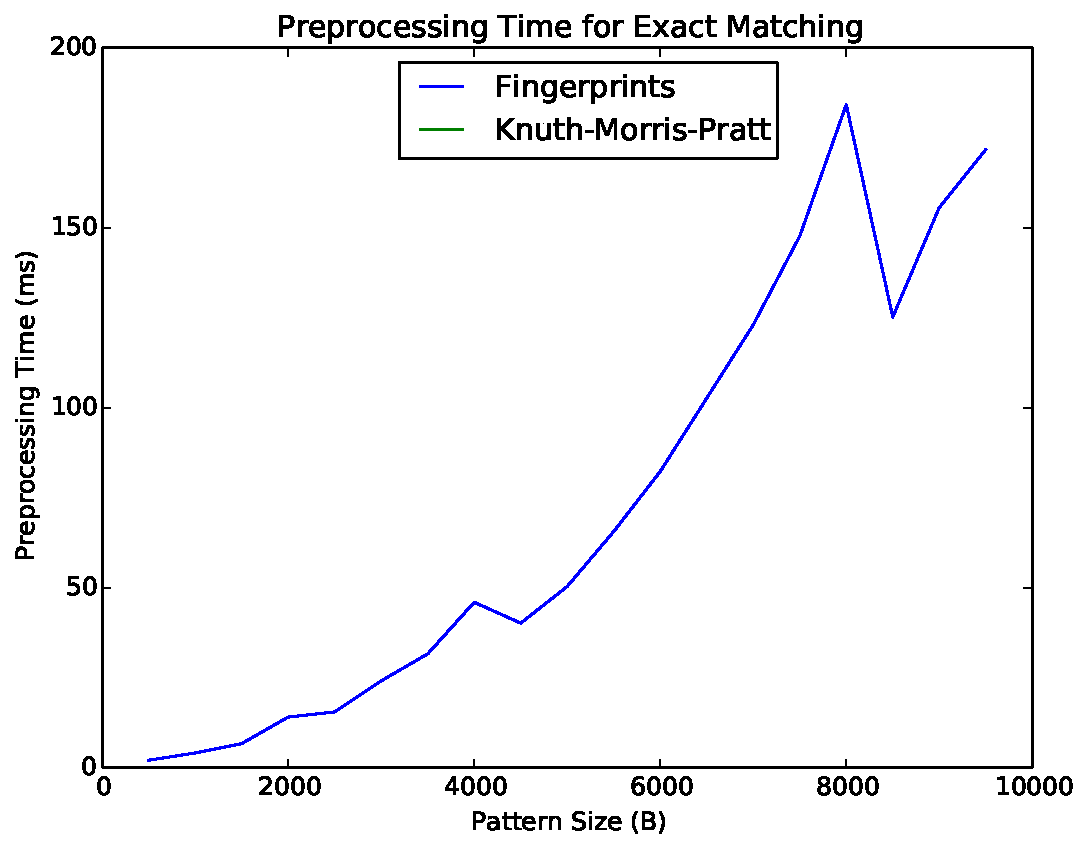
\includegraphics[width=0.5\linewidth]{summer_build_time}\\
  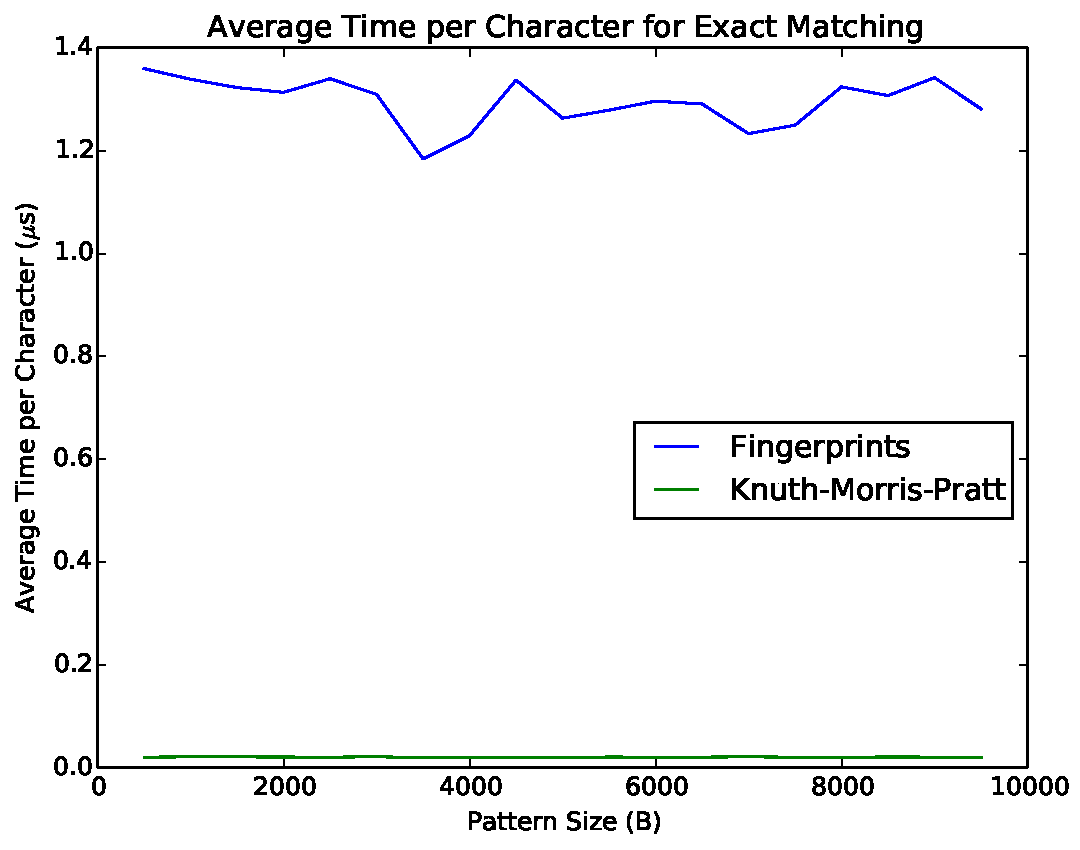
\includegraphics[width=0.5\linewidth]{summer_run_time}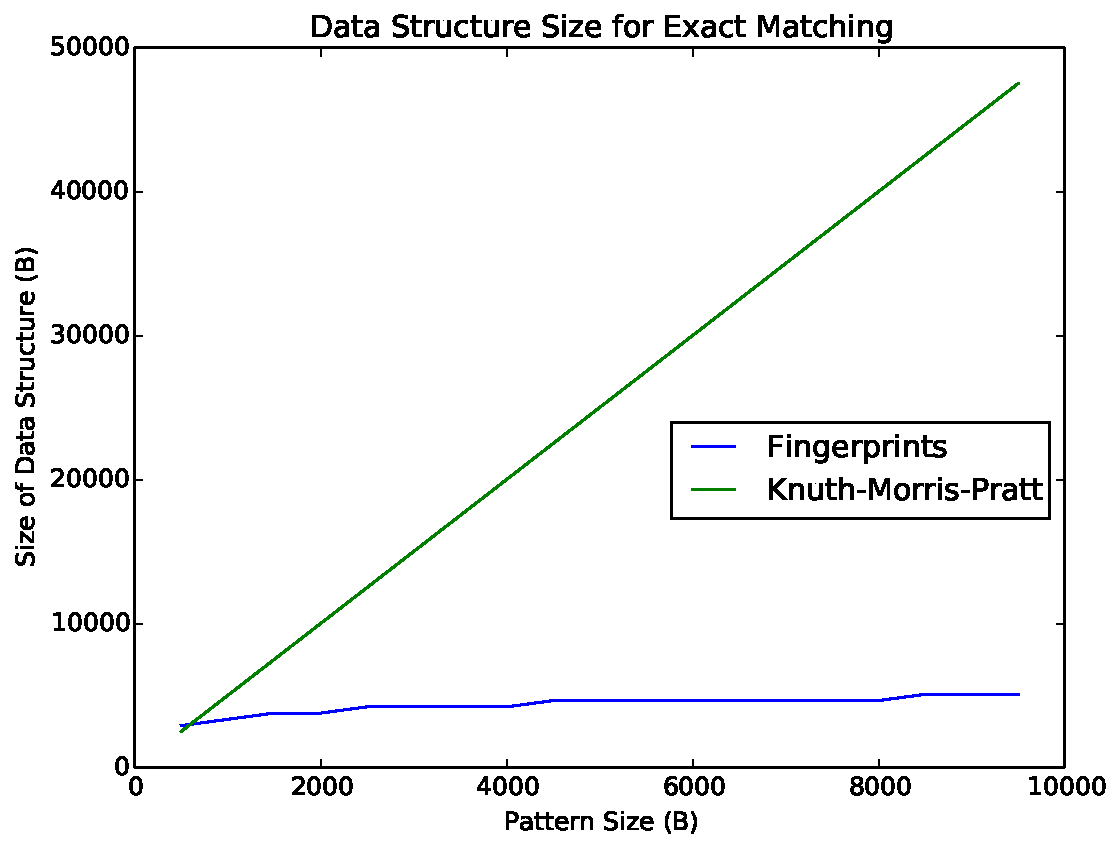
\includegraphics[width=0.5\linewidth]{summer_size}
\end{center}
\caption{Build time, run time and space performance for Breslauer and Galil's algorithm against Knuth-Morris-Pratt}
\label{fig:summer-results}
\end{figure}

\section{Clifford, Fontaine, Porat and Sach: Dictionary Matching in Sublinear Space}
\label{sec:theory-clifford}

Clifford et al.\cite{2015arXiv150406242C} provided a solution to dictionary matching under the streaming model in less space than it takes to store the pattern. Their solution uses $O(k\log m)$ space and $O(\log m)$ time per character, where $m = \max(M)$. It is worth noting that this description is based on a version of this paper that was not accepted, and the accepted version of the paper has some differences to what is described here. Also, please note that this is how the algorithm is described in the paper; any changes in later chapters are my own corrections.

The first step to understanding the algorithm as described in the paper is to consider a subset of the dictionary matching problem, where all the patterns are a power of two in length. This algorithm is very similar to the one described in Section~\ref{sec:porat-porat}, where all the patterns are broken up into $\log m_i$ fingerprints, denoted $\phi_{i,j}$ and defined as follows:

$$\phi_{i,j} = \phi(p_{i,0}...p_{i,2^j-1})$$

Each level of the algorithm now contains up to $k$ of these prefix fingerprints, and stores all of them in a static perfect hash table. Along with this, each level stores up to $k$ arithmetic progressions of viable occurrences. When the next character enters the stream, each level checks if one of the arithmetic progressions has a viable occurrence that requires processing. If there is, then the algorithm uses static perfect hashing to check if the last $2^j$ characters in the text match any of the prefixes at that level. If there is a match, that VO is promoted to the next level. Finally, a boolean is also specified in the hash table to indicate if the given fingerprint is actually the fingerprint of a whole pattern. If that boolean is True, then a match at that index is reported.

In terms of complexity, each level requires $O(k)$ space and there are $\log m$ levels, so space usage is $O(k\log m)$ as required. Time complexity depends on how long it takes to determine if an arithmetic progression needs processing and if so which one. Assuming this can be done in constant time, then each level takes constant time and thus an overall performance of $O(\log m)$ time per character is given.

In order to go from this to the general case of any length of pattern, the patterns are broken up into three cases, based on their length $m_i$ and period $\rho_i = \rho_{P_i}$:

$$|\rho_i| \geq k; (m_i \geq k \text{ and } |\rho_i| < k); m_i < k$$

\subsection{Patterns with Long Periods (Long Patterns)}
\label{ssec:long-theory}

We start with the case where for every pattern $P_i$ in our dictionary $|\rho_i| \geq k$. We start by defining $Q_i$ to be the $m_i - k$ prefix of the $i$-th pattern. For this algorithm to work, we continue under the assumption that $|\rho_{Q_i}| \geq k$. We will see a brief solution for when this assumption does not hold in Section~\ref{sssec:edge-case-theory}.

The first part of this case functions in the same way as the power of two length case. We perform the above algorithm on $\log|Q|$ levels, where $Q$ is the prefix of the longest pattern. If there is a match at a given level, we insert the viable occurrence into a special row, which stores one arithmetic progression for each prefix. At each text index $j$, we process two prefixes. Let $Q_i$ be one of those prefixes processed at $j$, and we perform the following:

\begin{enumerate}
  \item First, if $j \geq l + |Q_i|$, where $l$ is the location of the VO stored in the arithmetic progression related to $Q_i$, then we check if $\phi(t_{l+1}...t_{l+Q_i+1}) = \phi(Q_i)$. In other words, did the $|Q_i|$ characters following the VO location match the prefix?
  \item If there is a match, then we insert all the fingerprints for the $k$ length suffixes of all the patterns in the dictionary for which $Q_i$ is a prefix into a binary search tree (BST). The binary search tree is set up so that it will only be queried when the stream reaches index $l + |Q_i| + k$.
\end{enumerate}

Finally, the algorithm checks to see if any binary search trees need processing. If so, the algorithm takes the fingerprint of the last $k$ characters seen in the stream, and searches the BST to see if a match is found. If a match is found, then an entire pattern has been matched, and the index $j$ is returned.

In terms of time complexity, processing the power of two length prefixes costs $O(\log|Q|)$ time per character by simply substituting $m = |Q|$. The first step of processing each prefix takes constant time, but may be delayed by up to $\frac{k}{2}$ characters. The second step is more complicated, and in the worst case  --  where all the patterns have the same $m_i - k$ length prefix  --  will take $O(k\log k)$ time per character if implemented na\"{i}vely. However, because of our assumption that $\forall i, |\rho_{Q_i}| \geq k$, each prefix can only occur once every $k$ characters. This means that, amortised over $k$ characters, our time complexity becomes $O(\log k)$ time per character. Furthermore, this can be deamortised by inserting two suffixes into the BST per index, bringing our worst case time complexity for this step down to $O(\log k)$ per character. Steps 1 and 2 are both delayed by at most $\frac{k}{2}$ indexes each, so the overall delay will be at most $k$ indexes, within time for the BST to be processed. Finally, searching the BST takes $O(\log k)$ time. Putting all of this together gives us $O(\log|Q| + \log k)$ time per character, and because of our assumption that $\rho_Q \geq k$, this becomes $O(\log|Q|) \in O(\log m)$ time per character.

As for space usage, the power of two length prefixes uses $O(k\log|Q|)$ space. Storing the fingerprints of all the prefixes costs $O(k)$ space, as does storing lists of all the suffixes. To cater for both the $\frac{k}{2}$ delay in the first step of the prefix processing and searching for the fingerprint of the last $k$ characters in a BST, we store a circular buffer of the last $k$ fingerprints, which takes up $O(k)$ space. Finally, we may need up to $k$ binary search trees, and at any given time the total number of nodes across all BSTs is at most $k$, so this again is $O(k)$ space. This gives us an overall space usage of $O(k\log|Q|) \in O(k\log m)$ space.

\subsubsection{An Edge Case}
\label{sssec:edge-case-theory}

As previously mentioned, there is an edge case in the above algorithm if $\exists i \text{ such that } |\rho_{Q_i}| < k$. Any patterns which fall under this case can be processed by using the algorithm for long patterns with short periods described in Section~\ref{ssec:periodic-theory} to process their prefix $Q_i$. Any matches returned from this algorithm can be extended from $m_i - k$ to $m_i$ by a combination of fingerprinting and static perfect hashing.

\subsection{Long Patterns with Short Periods (Periodic Patterns)}
\label{ssec:periodic-theory}

The next case detailed is where the patterns in the dictionary are longer than $k$, but their periods are shorter. In this algorithm, we store a fingerprint of the $k$ length prefix of each pattern, and call the result $K_i$. For each $K_i$, we store a fingerprint of the period of the pattern $\phi(\rho_i)$ and the period's length $|rho_i|$, along with a counter of the number of times it has occurred, the index of the last time it occurred in the current arithmetic progression and the fingerprint of the text at the last occurrence.

When a new index comes in, we use a static perfect hash function to check if the fingerprint of the last $k$ characters in the text stream matches any $K_i$. If so, we determine if this index fits with the rest of $K_i$'s arithmetic progression by checking the current index is $|\rho_i|$ characters away from the last occurrence and if the difference between fingerprints of the current stream and the last occurrence matches the fingerprint of the period. If they do match then we increment the counter, otherwise we abandon the arithmetic progression by resetting the counter to 1 and setting the last occurrence to the current index and fingerprint.

The second step we perform is to check if the fingerprint of the last $k$ characters in the text matches the last $k$ characters in one of the patterns  --  referred to as the \textit{tail} of each pattern. This can be done by storing the fingerprint of the tails of each pattern in another static perfect hash table.

At this point, we are going to assume that no patterns are a suffix of another pattern. If this is not the case, then it is possible to perform dictionary matching, but it comes at the cost of not knowing which patterns have matched. Either way, we end up in a situation where each pattern has a unique tail. If the last $k$ characters in the stream match the tail of some pattern $P_i$, we check the arithmetic progression associated with that pattern. In order for a match to have occurred, there needs to have been at least $\lfloor\frac{m_i}{\rho_i}\rfloor$ occurrences of $K_i$ in the progression, and the last occurrence must have happened at index $j - m_i + \lfloor\frac{m_i}{|\rho_i|}\rfloor\cdot|\rho_i|$. If both of these conditions hold, then a match is reported.

Complexity wise, the progressions can be stored in $O(k)$ space, as can the fingerprints of the tails. The fingerprint of the last $k$ characters in the text stream can be computed by storing a cyclic buffer of text fingerprints for the last $k$ indexes. Thus space usage is $O(k)$. As for time, the static perfect hashing operations are constant time, as is inserting the occurrence into the arithmetic progressions and checking for a match, so time overall is $O(1)$.

\subsection{Short Patterns}
\label{ssec:short-theory}

The final case to consider is where all the patterns are shorter than $k$. The algorithm for this case is an adaptation of binary search, searching over suffixes of the stream of lengths from 1 to $k$ to see if a pattern matches any of them. However, binary search cannot be applied na\"{i}vely, as we may need to search both parts of the search space. Instead, we use a hash table with a fingerprint as the key and a boolean as the value to find out which half of the space to search.

Algorithm~\ref{alg:short-dict-matching} computes the hash table that is used. We call $\texttt{PreProc}(k',m_i)$ on each pattern $P_i$, where $k'$ is the nearest integer power of two no smaller than $k$. $\mathcal{S}$ is a boolean function which, given a string, returns True if there is a pattern in the dictionary which is a suffix of that string, and False otherwise.

\begin{algorithm}[t]
\uIf {$y \geq x/2$} {
  $\mathcal{H}_3.\text{insert}(\phi(p_{m_i-x/2}...p_{m_i}), \mathcal{S}(p_{m_i-x/2}...p_{m_i}))$\\
  $\texttt{PreProc}(x/2,y - x/2)$
}
\Else {
  $\texttt{PreProc}(x/2,y)$
}
\caption{$\texttt{PreProc}(x,y)$: Preprocessing of a single pattern}
\label{alg:short-dict-matching}
\end{algorithm}

At each index $j$, we keep a cyclic buffer of the previous $k'$ fingerprints of the whole stream. We start our binary search by seeing if $\phi(t_{j - k/2 + 1}...t_j)$ is within the hash table and its associated boolean value. If the boolean value is True; we know that there is an occurrence of the pattern which ends at this index, so we report it. If the boolean value is False but the key exists in the table, then we know that this fingerprint matches the suffix of a pattern, but not necessarily all of it, so we check the longer suffixes of the text. If there is no key in the table, then we know that no pattern matches this suffix, but a pattern might match shorter ones, so we check shorter suffixes instead. This continues until we either report an instance or run out of search space.

For space complexity, the only space used is the hash function which uses $O(k\log k)$ space to store the fingerprints and their associated booleans, and the cyclic buffer, which uses $O(k') \in O(2k) \in O(k)$ space, so the overall space usage is $O(k\log k)$. The only step in the algorithm is the binary search, which takes $O(\log k)$ time per character.

%-----------------------------------------------------------------------------

\chapter{Project Execution}
\label{chap:execution}

\section{Aho-Corasick}

\subsection{From Knuth-Morris-Pratt to Aho-Corasick}

As stated in Section~\ref{sec:aho-corasick}, Aho-Corasick\cite{Aho:1975:ESM:360825.360855} is a generalisation of Knuth-Morris-Pratt. Because of this, I decided the most suitable way to implement this algorithm was to start with an implementation of KMP and then generalise it to $k$ patterns.

Most implementations of KMP simply consist of an array of $m$ integers to act as a failure table, a string of $m$ characters for the pattern, and a counter of the number of characters that have matched so far, with the counter reaching $m - 1$ representing the accept state. But this is actually a simplification of the algorithm. As pointed out in CLRS\cite{clrs:kmp}, the correctness of Knuth-Morris-Pratt can be proven because this array, string and integer represent a finite state automaton: The array of integers represent the state the automaton should fall back to if the pattern does not match, the string shows the next character that needs to arrive in the text in order for the automaton to move one state closer to the accept state, and the counter represents the current state the automaton is in, with $m - 1$ being the accept state of the automaton.

We can show this with an example: Table~\ref{tab:kmp-pattern-failure} shows the pattern and failure table for the pattern $aabab$, and Figure~\ref{fig:kmp-pattern-failure} shows the state transition diagram for the same pattern.

\begin{table}[t]
  \centering
  \begin{tabular}{|l|c|c|c|c|c|}
    \hline
    \textbf{Index} & 0 & 1 & 2 & 3 & 4 \\\hline
    \textbf{Pattern} & $a$ & $a$ & $b$ & $a$ & $b$ \\\hline
    \textbf{Failure} & -1 & 0 & -1 & 0 & -1\\\hline
  \end{tabular}
  \caption{Pattern and failure table for pattern $aabab$}
  \label{tab:kmp-pattern-failure}
\end{table}

\begin{figure}[t]
  \centering
    \begin{tikzpicture}[node distance=2cm,on grid,auto]
      \node[state] (start) at (0,0) {-1};
      \node[state] (0) [right of=start] {0};
      \node[state] (1) [right of=0] {1};
      \node[state] (2) [right of=1] {2};
      \node[state] (3) [right of=2] {3};
      \node[accepting, state] (4) [right of=3] {4};
      \path[->]
        (start) edge node {$\{a\}$} (0)
        (0) edge node {$\{a\}$} (1)
        (1) edge node {$\{b\}$} (2)
        (2) edge node {$\{a\}$} (3)
        (3) edge node {$\{b\}$} (4)
        (start) edge [loop left] node {$\Sigma/\{a\}$} (start)
        (0) edge [bend left] node {$\Sigma/\{a\}$} (start)
        (1) edge [bend left] node {$\Sigma/\{b\}$} (0)
        (2) edge [bend right] node {$\Sigma/\{a\}$} (start)
        (3) edge [bend left] node {$\Sigma/\{b\}$} (0.south)
        (4) edge [bend left] node {$\Sigma$} (start.south);
    \end{tikzpicture}
  \caption{State transition diagram for pattern $aabab$. Edges directed right represent matches, edges directed left represent failures.}
  \label{fig:kmp-pattern-failure}
\end{figure}

The first important decision was how to implement the automaton. As a finite state automaton is based on graphs, there were three main options available:

\begin{itemize}
  \item \textbf{Adjacency Matrix:} An item at coordinates $(i,a)$ in the matrix represents an edge in the matrix from state $i$ if the next character is $a$. The value of $(i,j)$ itself is the \texttt{goto} state, and is set to the failure state if there is no subsequent pattern with the next character in the state. This takes constant time travelling between states but $O(m|\Sigma|)$ space.
  \item \textbf{Adjacency List:} Each item in the list is a tuple $(i, j, a)$, representing an edge from $i$ to $j$ if $a$ is next on the tape. Failure edges are represented by an integer for each state. This requires potentially less space than an adjacency matrix but $O(m \min(|\Sigma|, m))$ time to move to \texttt{goto} state.
  \item \textbf{Object Oriented:} A state structure is defined, with an array of pointers to other states it connects to and the next character that needs to be read on the tape for the automaton to enter that state. Failure edges are simply a pointer to failure state. The ferformance is a compromise between an adjacency matrix and an adjacency list, with the same asymptotic space consumption as an adjacency list but $O(\min(|\Sigma|, m))$ time to move to \texttt{goto} state.
\end{itemize}

My initial decision was to use the object oriented approach. Implementing Knuth-Morris-Pratt in this form is easy: When constructing the \texttt{goto} edge, we just iterate through each character in the pattern and connect a new state to the most recent state made. When both constructing the failure pointer and processing the text, we just use the standard KMP algorithm, only using pointers to states instead of integers. And when destroying the automaton at the end, we just recursively call the destroy function on the \texttt{goto} item in the automaton. Note that we don't worry about destroying the node pointed to along the failure edge, as we know that will be destroyed later.

However, while this method was simple enough for KMP, generalising it for Aho-Corasick led to a number of memory problems. In particular, there were issues with the starting state of the automaton being overwritten by another node later on, leading to corrupted memory and double free attempts. The conclusion was that this was too problematic an implementation of automaton for C.

In the end, a hybrid method was used for representing the automaton, combining adjacency matrices with the object oriented approach. The current state is simply represented by an integer, the \texttt{goto} state is represented by a 2-D array of integers \texttt{goto}, the character it needs to match is represented by an array of strings \texttt{match} and the failure edges represented by an array of integers \texttt{failure}. Thus if we're in state $i$ and character $a$ is the next character in the text, the next state we move to is determined by:

\[
  \begin{cases}
    \texttt{goto}(i, j),& \text{if } \exists j \text{ such that } \texttt{match}_i(j) = a\\
    \texttt{failure}(i),& \text{otherwise}
  \end{cases}
\]

This has the same performance as the object oriented approach, both in terms of time and space.

One detail to remember is that the current state is the index of several arrays. Thus, we cannot have our start state as -1 anymore. This is easy to remedy, by replacing the start with 0. This is the only discrepancy between our terms for KMP above and our work on Aho-Corasick below.

\subsection{Removing the $\Sigma$ Dependency from Preprocessing}
\label{ssec:ac-hashing}

One of the major problems with the Aho-Corasick algorithm as it is defined in Section~\ref{sec:aho-corasick} is that Algorthms~\ref{alg:ac-goto}, \ref{alg:ac-failure} and \ref{alg:ac-next} all rely on knowing the complete alphabet at preprocessing time. This is not guaranteed under the streaming model, and requires multiple passes over the text and pattern.

In order to cater for this, a few changes have been made to each algorithm. For Algorithm~\ref{alg:ac-goto}, we change it by specifying the result the output from \texttt{goto} if the next character does not match $failure = 0$. This removes the need for the final loop entirely on that case.

For Algorithm~\ref{alg:ac-failure}, we already know for every state $i$ every character $a \in \Sigma$ such that $\texttt{goto}(i, a) \neq fail$, because all of these characters are stored in the \texttt{match} strings, so we can simply iterate through each state's associated string.

It is hardest to remove the alphabet dependency from Algorithm~\ref{alg:ac-next}, but it is still achievable. For the first loop, we only iterate over the characters in state 0's $\texttt{match}_{0}$ string, and set $\texttt{next}(i, a) = 0$ by default. For any other state, denoted $i$, we start by handling the case where $\texttt{goto}(i, a) \neq fail$, by simply iterating through the characters stored in the $\texttt{match}_i$ strings. We then handle the other case by iterating through every character $a \in \texttt{next\_chr}_{\texttt{failure}(i)}$, where $\texttt{next\_chr}_i$ is the string of characters for state $i$'s \texttt{next} function: if $a \notin \texttt{match}_i$, then we know that $\texttt{goto}(i, a) = fail$. If $\exists a \in \Sigma \text{ such that } a \notin \texttt{match}_i \cup \texttt{next\_chr}_{\texttt{failure}(i)}$, it must hold that $\texttt{next}(i, a) = 0$, as it does by default, so we do not need to worry about these characters.

\subsection{Removing the $|\Sigma|$ Run Time per Character}

The bottleneck with Aho-Corasick at processing time is that for our current state, we need to compute the \texttt{next} function. This is not easy to implement; the simplest implementation is linear search, as described in Algorithm~\ref{alg:ac-search}, which would take $O(|\Sigma|)$ time per character. A more efficient implementation could use a binary search tree, which would be $O(\log|\Sigma|)$, but there is in fact an even better way.

\begin{algorithm}[t]
\For{$i=0$ {\bf upto} $|\texttt{next\_chr}_i|$}{
  \If{$\texttt{next\_chr}_i(j) = a$}{
    {\bf return} $\texttt{next\_state}_i(j)$
  }
}
{\bf return} 0
\caption{Computing the $\texttt{next}(i, a)$ function by linear search.}
\label{alg:ac-search}
\end{algorithm}

After preprocessing, we never add any characters to or remove any characters from $\texttt{next\_chr}_i$. As a matter of fact, the \texttt{next} function does not change at all after preprocessing has completed. This means that we can compute this function by having a static perfect hash table for each state $i$, with $\texttt{next\_chr}_i$ as the keys and $\texttt{next\_state}_i$ as the values. This gives us constant time per character.

For implementation, I used the C Minimum Perfect Hashing Library (CMPH) configured to the Compress, Hash and Digest algorithm (CHD). This was contained in a data structure based on my summer project as mentioned in Section~\ref{sec:summer}. One of these three cases occurs when a structure is searched with key $key$:

\begin{enumerate}
  \item If there are no keys and values for a hash table, return 0 by default.
  \item If there is one key, check if $keys_0 = key$ and if so return $values_0$, if not return 0.
  \item Otherwise, do a CMPH search on the key. If none of the keys match the search key, CMPH will by default return either the number of keys or the index of some key. If it returns the index of some key $i$, check if $keys_i = key$. If they match, return $values_i$, otherwise return 0.
\end{enumerate}

Because the keys are a single character, each search can be evaluated in constant time. Since we are implementing the \texttt{next} function, we only need to call one search per index. Thus the overall run time per character for the algorithm is now constant time. The hash function takes up the same amount of space as the \texttt{next} function would, as does the rest of the search structure, as we are using a minimum perfect hash function. There are only as many search structures are there are states, so we are left with the same space usage as traditional Aho-Corasick.

\subsection{A Brief Note on \texttt{output}}

Aho-Corasick offers the advantage that we can return the patterns which were matched at a given index. However, for this project, we only care about \textit{if} a pattern matched, regardless of \textit{which} patterns matched. Because of this, the \texttt{output} function was changed from returning a set to returning an integer, with 0 to represent no patterns matching and 1 to represent a match.

This change requires two lines of the algorithm being modified:

\begin{enumerate}
  \item Line 15 of Algorithm~\ref{alg:ac-goto} becomes $\texttt{output}(state) = 1$
  \item Line 15 of Algorithm~\ref{alg:ac-failure} becomes $\texttt{output}(state) = \texttt{output}(state) \vee \texttt{output}(\texttt{failure}(state))$
\end{enumerate}

If unspecified, $\texttt{output}(state)$ is 0 by default.

\section{Power of Two Length Patterns}

The rest of this chapter describes the implementation of Clifford, Fontaine, Porat and Sach's\cite{2015arXiv150406242C} algorithm as described in Section~\ref{sec:theory-clifford}. Note that this implementation does not achieve $O(\log m)$ time per character as desired, but $O(\log k\log m)$ instead. The reason behind this will be explained later in this section. It is also worth noting, as will be explained in Section~\ref{ssec:static-hash-fail} that in the general case this is amortised time per character; the real time per character is $O(\log k(k + \log m))$. A method for deamortising the solution will be proposed in Section~\ref{ssec:deamortise}.

\subsection{Implementing Karp and Rabin's Algorithm for Dictionary Matching}

My first choice for implementation was to investigate the algorithm described in Section~\ref{sec:kr-fingerprints} for dictionary matching when all patterns are the same length, based on Karp and Rabin's original algorithm. This is because it is a simpler algorithm to implement than Clifford et al., yet both require similar libraries: One for static perfect hashing and one for Karp-Rabin fingerprints.

Using these libraries, implemented as described in the two sections below, Karp and Rabin's algorithm was straightforward to implement. The static perfect hash function contained fingerprints of all the patterns. We stored and updated a fingerprint of the last $m$ characters by concatenation and suffix operations using a circular buffer of the last $m$ characters. This offers $O(k + m)$ space and $O(1)$ time per character, as mentioned before.

\subsubsection{Implementing Karp-Rabin Fingerprints}
\label{sssec:kr-implementation}

The library for Karp-Rabin fingerprints was written using the GNU Multiple-Precision Arithmetic Library (GMP) version 6.0.0 for the C programming language.

There are two reasons for using GMP:
\begin{enumerate}
  \item It allows for fingerprints and primes to be of any size.
  \item Picking a prime number is fast and doesn't require implementation itself, due to the \texttt{mpz\_nextprime} function.
\end{enumerate}

The downside is that multiple precision operations are typically slower than standard 32/64-bit arithmetic. It was decided that this was a worthwhile cost, as we required the ability to process large amounts of data.

The library itself was based on my summer project described in Section~\ref{sec:summer}, and consisted of two structures as described below.

The first structure, called a fingerprinter, consists of two multiple precision integers $p$ and $r$. When initialised, the fingerprinter takes as input the length of the text $n$, uses GMP to work out $n^2$ and then $\texttt{mpz\_nextprime}(n^2)$ to pick a prime number $p$.

The integer $r$ is where this library most significantly differs from my summer project. For both implementations, entropy is gathered by reading in data from \texttt{/dev/urandom} and then used to seed the GMP pseudorandom number generator. For the summer project, the integer $r$ was picked using the Mersenne Twister function on \texttt{mpz\_urandomm} with maximum value $p$. But this is not guaranteed to work, as it allows two problematic cases:

\begin{itemize}
  \item If $r = 0$, then $\phi(S) = \phi(S')$ if $s_0 = s'_0$.\footnote{If the fingerprints are implemented exactly as described in Section~\ref{sec:kr-fingerprints}, then $\phi(S)$ will always match $\phi(S')$. This difference is due to my implementation of the fingerprints, which assumes $r^0 = 1$ and thus simply uses $\phi(s_0) = s_0$.}
  \item If $r = 1$, then $\phi(S) = \phi(S')$ if $S$ is a reordering of the characters in $S'$.
\end{itemize}

To avoid these two cases, \texttt{mpz\_urandomm} is still used, but the maximum is now set as $p-2$. This will generate a number $r$ such that $0 \leq r < p-2$. Incrementing $r$ by 2 gives us $2 \leq r < p$. This means that the fingerprints will not work if $p = 2$, but this is only the case if $n = 1$, in which case the text is one character long and can just be matched na\"{i}vely.

The second structure, called a fingerprint, consists of three multiple precision integers: \texttt{finger} refers to the fingerprint of the string itself $\phi(S)$ for a $k$ character string $S$, \texttt{r\_k}, which refers to $r^k$, and \texttt{r\_mk}, which refers to $r^{-k}$.

After space has been allocated, the fingerprints of strings can be computed by a function called \texttt{set\_fingerprint}. This function is implemented as the equation in Section~\ref{sec:kr-fingerprints}, and based on the work from my summer project. However, there was a problem with my summer project's implementation, where the first item was not being computed modulo $p$. This meant that, if the string $S$ was 1 character long and $s_0 \geq p$ -- a case which is easily possible depending on the encoding of the characters in the string and if $p$ is sufficiently small -- then $\phi(S) \geq p$. This was easily fixed by adding an additional modulo operation on the first character of the string. $r^k$ was calculated incrementally as $r\cdot r\cdot r\cdot ...\cdot r$, as we required $r^0,r^1...,r^{k-1}$ for computing the fingerprint, and $r^{-k}$ was calculated using \texttt{mpz\_invert} on $r^k$.

Concatenation, prefix and suffix operations are computed as shown in Section~\ref{sec:kr-fingerprints}. The only difference is that, as with setting the fingerprint, $r^{-k}$ was calculated using \texttt{mpz\_invert}.

\subsubsection{Implementing Static Perfect Hashing of Fingerprints}
\label{sssec:static-hashing-kr}

The data structure is similar to the static hash table used for Aho-Corasick, only with fingerprints instead of characters for the keys, and returning the index calculated by the hash function (or $-1$ by default) instead of some value. But there is a problem with this method: The C version of CMPH\footnote{The C++ version, in comparison, can handle any type.} is designed to take strings alone as keys, whereas we want it to run on (multiple precision) integers.

The method for solving this problem was to convert the fingerprints into strings, using the function \texttt{gmp\_snprintf}. While this could impact performance, it was a quick solution to make static hashing work on integers. Our conclusion was that if it becomes a bottleneck at the testing stage, faster implementations of static hashing could be further investigated or suggested as future work.

The fingerprints were converted into hexadecimal strings in order to simplify calculating the maximum length. \texttt{gmp\_snprintf} was used specifically to avoid any chances of a buffer overflow, as we specify the maximum number of characters to write to the string. The maximum length of the string was calculated based on the hexadecimal representation of the modulus $p$, since all fingerprints were integers between 0 and $p - 1$ inclusively.

We cannot determine the number of characters needed to represent $p$ in hexadecimal exactly without testing individual bytes of $p$, but we can approximate it. Because $p$ is a positive multiple-precision integer from GMP, the number of limbs used to represent $p$ is specified by the integer \texttt{\_mp\_size}. We can multiply this value by $\texttt{sizeof}(\texttt{mp\_limb\_t})$ to get an upper bound on the number of bytes required to represent $p$. Finally, because a byte can be represented by two hexadecimal digits, we double this size, and allocate an extra character at the end for the string terminator \texttt{`\textbackslash0'}.

Asymptotically, the space is not affected by this change. We only need to store one string in the structure for the key we want to search at a given point -- we store this string in order to avoid constantly allocating and freeing space -- and this string will take up as much space as $p$, within a constant factor.

\subsection{From Karp-Rabin to Power of Two Length Dictionary Matching}

\subsubsection{Dictionary Matching Where All Patterns are the Same Power of Two Length}

The next step of implementation was to look at patterns which are all the same power of two length. This essentially works as a combination of Porat and Porat's algorithm with the Karp-Rabin algorithm implemented in the previous section.

The first step is to determine the length of the longest pattern $m$, and then use this to compute $\log m$, so that we can allocate enough rows for the pattern. This is straighforward: Iterate through all of the pattern lengths to find the longest, and use bit shifting to compute $\log m$.

Because the very first row, which matches prefixes one character long, doesn't need any arithmetic progressions stored, we just process those characters live as they come in on the stream. Thus we actually only need $\log m - 1$ rows. For this reason, we handle the first row differently. Instead of having an array of progressions for it, we have a static hash table to check each character $t_j$ as it enters the stream to determine if it matches the prefix of some pattern, and then insert it into level 0 if there is a match. We don't use the fingerprint static hash table described above for these prefixes. Instead, because these prefixes are only one character long, we use the static hash table used in Section~\ref{ssec:ac-hashing}, which is faster than hashing $\phi(t_j)$.

The rest of the structure is built by iterating through each row $i$ until $2^{i+1} = m$, which occurs when $i = \lfloor\log_2m\rfloor$. For row $i$, we iterate through each pattern $P_j$ and create the fingerprint $\phi_{i,j} = \phi(p_{j,0}...p_{j,2^{i + 1} - 1})$. As with Porat and Porat in Section~\ref{sec:porat-porat}, this fingerprint can be created reading each character only once by concatenating the previous prefix with $\phi(p_{j,2^{i}}...p_{j,2^{i + 1} - 1})$.

One point to be cautious about, is if different patterns have the same prefix. This can cause problems with CMPH, which does not handle matching keys well, and can also cause later problems for us when looking at patterns of different lengths, if one entire pattern is the prefix for another pattern. We will see this problem arise regularly throughout this project, as all three cases described later in this chapter have the risk of matching fingerprints. In all cases where this issue arises during preprocessing, avoiding this is implemented na\"{i}vely through linear search to check for duplicates. A better option would have been to implement it via a binary search tree, but this was only realised after testing was completed.

For each row $i$, we keep count of the number of unique prefixes in that row. We need this information so that when we start building row $i+1$, we know how many arithmetic progressions need to be allocated. For this implementation, it does not matter which prefix in row $i$ maps via CMPH to which progression in row $i+1$.

This concludes preprocessing. The rest of the algorithm works similarly to the description in Section~\ref{sec:theory-clifford}: As each character of the text enters, each row is checked to determine if the oldest occurrence stored in any progression can now be tested. If it is tested and succeeds, then it is promoted to the next row and stored using the prefix's period. A few differences are explained below.

Firstly, we do not promote at the final level. Instead, since the final level performs matches against the complete patterns, this level performs a static lookup to see if a full match has occurred and if so reports that match.

The second and more complicated difference is what to do if there is a collision in the fingerprints and thus there is a viable occurrence that does not fit with the period. We could use the method suggested by Breslauer and Galil in Section~\ref{sec:porat-porat} and simply report a match every time this happens, but this will cause problems once the patterns are of different lengths since we will not know at which index to declare a match. Instead, this implementation simply ignores such occurrences, and prints a warning on \texttt{stderr} explaining that there was a non-periodic occurrence at this index, which prefix causes the occurrence, and that it has been ignored.

The final difference is how we figure out which arithmetic progression contains the oldest viable occurrence. This detail was omitted from the version of the paper that I was using for this project, and a method for solving this was not devised until it was too late to attempt to implement it. In the original implementation, a simple linear search was performed over the progressions. But this is too costly, as it makes the run time per character to $O(k\log m)$. With that level of asymptotic performance, we gain no benefit over merely running $k$ copies of the Breslauer and Galil algorithm described in Section~\ref{ssec:breslauer-galil}.

Instead, the next progression was found by using a Red-Black Tree, using source code from \url{http://en.literateprograms.
org/Red-black_tree_(C)?oldid=19567} as a starting point. More precisely, I used a version from my summer project which modified the RBT source code so that when searching the tree, a default value could be specified if the key could not be found. This is because the original implementation of the RBT returns \texttt{NULL} by default, which is problematic as \texttt{NULL} is interpreted by C as 0, and I want to store the value 0 in the tree.

Each row has an RBT as part of its data structure, which takes integers as both keys and values. For key-value pair $i, j$ in a tree, $i$ is the index of the oldest prefix in the $j$-th progression that is yet to be tested. When a viable occurrence is added to an arithmetic progression, a key-value pair is added to the RBT only if that progression was previously empty. Then, when we reach index $i$ in the text, we check the RBT if one of the keys in the tree matches $i$. If so, then progression $j$ can be tested. After testing, we remove $i$ from the RBT, and if the progression $j$ still contains some viable occurrences, insert $(i + |\rho_j|, j)$ into the tree, where $|\rho_j|$ is the length of the period of the $j$-th progression.

There are a few final points worth noting about these trees. Firstly, because the prefixes are the same length, it is impossible to have more than one progression to test for a given index. Thus we have no risk of progressions being lost because of other progressions overwriting them in the RBT. Secondly, because we only insert items into the tree if either the progression was previously empty or because we have shifted the progression along -- which involves deleting an item from the RBT -- we have at most $k$ items in the tree at any one time. Thus, we still meet the $O(k\log m)$ space bounds as before.

As for time complexity, inserting, searching and deleting items from the red-black tree take $O(\log k)$ time, where $k$ is the number of items in the tree. We call these functions a constant number of times for each level at each index of the text. Because there are $\log m$ levels to iterate over at each index of the text, the overall runtime is $O(\log k\log m)$, as mentioned at the start of this section.

\subsubsection{Dictionary Matching with Different Power of Two Length Patterns}

From the above implementation, modifying it to handle patterns of different power of two lengths is trivial. For each level, we keep track of an array of integers to indicate if a pattern ends at a given prefix. When preprocessing on pattern $P_j$ at level $i$, we check if $2^{i + 1} = m_j$. If that is the case, then we specify a pattern ending in the array by the value $1$. Otherwise, we use $0$ to indicate that the pattern does not end here. To cater for the case where one pattern is the prefix of another and thus have matching fingerprints, we simply use a bitwise OR to make sure that the array knows that a pattern ends at this prefix.

Finally, the static perfect hash table\footnote{Note that this refers to both the hash tables for fingerprints and the hash table for characters in the first level.} is modified to store these integers, and optionally return them by reference.

Now for each character in the text, we iterate over each level and use the static hash table to check if there is a match with some prefix. In addition, we are returned by reference an integer to indicate if a complete pattern matches. If the integer is 1, we report a match at this index, otherwise we report no match.

\section{Prelude to the General Case Algorithms}

Sections~\ref{sec:impl-short}, \ref{sec:impl-periodic} and \ref{sec:impl-long} look at implementing each of the three algorithms by Clifford et al. described in Section~\ref{sec:theory-clifford} for the general case of dictionary matching. This section is for general points applied to all three algorithms.

The algorithms are described in this report in opposite order from how they are described in the original paper. This is intentional, as this was the order I implemented each algorithm in.

\subsection{Redefining the Cases for Each Algorithm}

Alongside the edge case described in Section~\ref{sssec:edge-case-theory}, there is a second case not considered by the paper. Consider a pattern $P_i$ of length $m_i = \frac{3k}{2}$ and period $\rho_i$ such that $|\rho_i| > k$. Because the pattern has a longer period than $k$, it should be processed by the algorithm described in Section~\ref{ssec:long-theory}.

Let $Q_i$ be the $m_i - k$ length prefix as previously defined. It is easy to see that $|Q_i| = \frac{3k}{2} - k = \frac{k}{2}$, and because $|Q_i| < k$, it follows that $|\rho_{Q_i}| < k$. So this hits an edge case that, according to the paper, should be fixed as described in Section~\ref{sssec:edge-case-theory}. But that means running the algorithm described in Section~\ref{ssec:periodic-theory} on $Q_i$, which will not work either as that algorithm relies on patterns being longer than $k$, which doesn't hold.

So we have another edge case. However, this one can be more easily rectified. Since this edge case occurs if the patterns are shorter than $2k$, we can simply process them using the algorithm for short patterns. We can state this change formally by a simple adjustment:

\begin{itemize}
  \item \textbf{Patterns with Long Periods:} $m_i > 2k \text{ and } |\rho_i > k|$
  \item \textbf{Long Patterns with Short Periods:} $m_i > 2k \text{ and } |\rho_i \leq k|$
  \item \textbf{Short Patterns:} $m_i \leq 2k$
\end{itemize}

The other difference between the definitions here and in Section~\ref{sec:theory-clifford} is that the equals conditions have been switched. This was for convenience, as this was the order I implemented the algorithms in. The correctness of all three algorithms still hold.

Note that the edge case -- defined under these new definitions as pattern $P_i$ of length $m_i$ with $(m_i - k)$-length prefix $Q_i$ such that $m_i > 2k \text{ and } |\rho_i > k|$ but $|\rho_{Q_i} < k|$ -- has not been implemented. This was due to time constraints, and the belief that this case was unlikely enough that efforts would be better focused elsewhere in this project.

\subsection{Determining the Period of Each Pattern}

The period length of each pattern can be determined by computing the Knuth-Morris-Pratt failure table for each pattern. Since the final element in the KMP failure table is the length of the longest strict prefix of the pattern that is also a suffix, the difference between that value and the length of the pattern is the point when the pattern starts repeating itself. Thus, we can get the period for each pattern by computing $|\rho_i| = m_i - \texttt{failure}_{m_i - 1} - 1$. The -1s are to cater for zero-indexing. To avoid too many memory allocation calls, the failure table is re-used for each pattern and only reallocated if the next pattern is longer than any previous ones.

\subsection{Re-using Buffers}

All three algorithms use a circular buffer of the last few fingerprints of the text. For the cases where the patterns have long periods or are long patterns with short periods, both algorithms use such a buffer of length $k$, and thus a buffer can be shared trivially. However, the short patterns algorithm uses a buffer of length $k'$ as described in the paper. I will describe in Section~\ref{sec:impl-short} how to adjust the algorithm in such a way that all three algorithms can use the same buffer.

It can also be seen that, following this redefinition, the buffer will now need to be of length $2k$ for the case of short matching. It will also be shown in each of the following sections how to adjust the algorithms for this longer buffer.

For implementation, a circular buffer is not used itself. Instead, a standard array of $2k$ fingerprints have been used instead. The oldest fingerprint at index $j$ is $j \mod 2k$ and serves as the start of the buffer. At the end of the computation for index $j$, the fingerprint at index $j \mod 2k$ is updated to the fingerprint of the whole text seen so far.

\section{Short Patterns}
\label{sec:impl-short}

\subsection{Modifications to the \texttt{PreProc} Algorithm}

There is in fact a typographical error in the way the \texttt{PreProc} algorithm is presented in the original paper -- see Algorithm~\ref{alg:short-dict-matching}. We can see this error if, for example, $P_i = aaaaa, m_i = 5, k' = 8$, as displayed in Table~\ref{tab:preproc-results-incorrect}. The problem is that it only inserts the power of two length suffixes into the hash table, so if our pattern is not a power of two in length, the full pattern will not be inserted.

\begin{table}[t]
  \centering
  \begin{tabular}{|c|c|c|c|}
    \hline
    Iteration & $x$ & $y$ & $p_{i, m_i-x/2}...p_{i, m_i - 1}$ \\\hline
    0 & 8 & 5 & $aaaa$ \\\hline
    1 & 4 & 1 & n/a \\\hline
    2 & 2 & 1 & $`a'$ \\\hline
    3 & 1 & 1 & $`'$ \\\hline
    4 & 0 & 0 & $`'$ \\\hline
  \end{tabular}
  \caption{Suffixes added to the hash table for pattern $aaaaa$ following \texttt{PreProc} as described in Algorithm~\ref{alg:short-dict-matching}.}
  \label{tab:preproc-results-incorrect}
\end{table}

It is easy to see that this is merely a typo as opposed to an error in the algorithm, as the algorithm can be simply fixed by modifying line 2 to the following:

$$\mathcal{H}_3.insert(\phi(p_{i, y - x/2}...p_{i, m{i} - 1}), \mathcal{S}(p_{i, y - x/2}...p_{i, m{i} - 1}))$$

This guides the algorithm to preprocess the patterns in the same order that binary search will traverse them, and essentially lay out the path for binary search to a given pattern.

The second modification was because the algorithm doesn't yet specify a base case for the recursive call to stop. The base case was in the end specified as $x = 0$, but checking this becomes problematic as in some cases we still want the algorithm to run when $x = 0$ in order to get a fingerprint of the entire pattern. So at the end of the recursive call, the entire pattern is inserted into the hash table.

The third modification is to simplify the algorithm. We can see from Algorithm~\ref{alg:short-dict-matching} that the value $x$ is never used, only $x/2$. So we can replace the occurrences of $x/2$ with $x$ and run $\texttt{PreProc}(k'/2, m_i)$ instead.

The final adjustment is to remove the recursive call. Because of how simple the recursion is, it is easy to convert the recursive call into a while loop and thus save the practical cost of recursion in time and stack space.

The completely modified algorithm is described in Algorithm~\ref{alg:preproc-correct}. We call \texttt{PreProc} with parameters $(k'/2, m_i)$ for each pattern $P_i$. The result of preprocessing this algorithm can be seen in Table~\ref{tab:preproc-results-correct}.

\begin{algorithm}[t]
\While {$x \neq 0$} {
  \If {$y \geq x$} {
    $\mathcal{H}_3.\text{insert}(\phi(p_{y-x}...p_{m_i}), \mathcal{S}(p_{y-x}...p_{m_i}))$\\
    $y \gets y - x$
  }
  $x \gets x/2$
}
$\mathcal{H}_3.\text{insert}(\phi(p_0...p_{m_i}), 1)$
\caption{$\texttt{PreProc}(x,y)$: Modified version of the algorithm for preprocessing of a single pattern}
\label{alg:preproc-correct}
\end{algorithm}

\begin{table}[t]
  \centering
  \begin{tabular}{|c|c|c|c|}
    \hline
    Iteration & $x$ & $y$ & $p_{i, m_i-x/2}...p_{i, m_i - 1}$ \\\hline
    0 & 4 & 5 & $aaaa$ \\\hline
    1 & 2 & 1 & n/a \\\hline
    2 & 1 & 1 & $aaaaa$ \\\hline
    3 & 0 & 0 & $aaaaa$ \\\hline
  \end{tabular}
  \caption{Suffixes added to the hash table for pattern $aaaaa$ following \texttt{PreProc} as described in Algorithm~\ref{alg:preproc-correct}.}
  \label{tab:preproc-results-correct}
\end{table}

Another point worth mentioning is how the function $\mathcal{S}$ is computed. For a string $S$ of $m$ characters, we iterate through every pattern in the dictionary $P_i$ and check if $m_i \leq m$. If that check holds, we then use na\"{i}ve pattern matcing to check if $s_{m - m_i}...s_{m - 1} = P_i$. This was the easiest solution to implement, and we can see at testing whether or not this is a bottleneck of the algorithm.

\subsection{Adjusting for Patterns Shorter than $2k$}

The above preprocessing changes will work for patterns shorter than $k$, but what about patterns shorter than $2k$? Thankfully, this adjustment can be made by simply modifying $k'$ to become the smallest power of two greater than or equal to $2k$. Because of how generic the \texttt{PreProc} and $\mathcal{S}$ functions are, the only adjustments needed to make them work for any patterns shorter than some length $c$ is to adjust $k'$ to be the smallest power of two greater than $c$.

So preprocessing works fine. But what changes need to be made to the streaming algorithm itself? Again, the answer is not a lot. The cyclic buffer needs to be modified to store the past $2k$ fingerprints of the text, and the initial position we check is $k'/2$ where $k'$ is defined by the new definition in the previous paragraph.

The final time and space constraints are the same as before, only with $2k$ substituted for $k$. Asymptotically, this is still the same overall complexity, as $O(2k) \in O(k)$.

\subsection{Reducing the Size of the Buffer}

The algorithm as described in Section~\ref{ssec:short-theory} uses a buffer of the last $k'$ fingerprints of the text. This is problematic if we want to share a buffer between all three algorithms, as the other two algorithms work with a buffer of $k$ fingerprints.

To solve this, it is worth investigating how \texttt{PreProc} behaves on a pattern $P_i$. In particular, note that the longest fingerprint inserted into the hash table is of length $m_i$; all other fingerprints have to be suffixes of the pattern and are thus shorter than $m_i$. We also know that all patterns are at most length $2k$ because of our definition of the problem. Thus, we can conclude that the maximum length of the strings stored in the static hash table is $2k$. Since we know that no strings will be in the hash table longer than this length, we don't need to check the hash table in this case and can just traverse right if we have a midpoint longer than $2k$. With this change applied to the binary search, we only ever compute the fingerprint of the last $2k$ suffixes in the pattern, so we can share this buffer with the other two algorithms.

\subsection{Why the Probability of Collisions Does Not Hold}
\label{ssec:short-collisions}

I mentioned at the end of Section~\ref{sec:kr-fingerprints} that the probability of two fingerprints colliding does not hold for this algorithm. This is because of the static hash table used here.

Recall that the probability of $\phi(u) = \phi(v)$ for different strings $u, v$ of length $l \leq n$ is smaller than $\frac{1}{n^{1 + \alpha}}$ as long as the fingerprint parameters $p, r$ are chosen correctly. Unfortunately, this probability does not hold for the hash table, which contains strings of different lengths. This makes the probability of collisions in the fingerprints significantly higher, to the point that this was the only point in the algorithm where I was actually seeing the hash function colliding.

We can resolve this by comparing more than just the fingerprints. For strings $u, v$ of respective lengths $l_u, l_v \leq n$, we define their fingerprints as being equivalent if the following equation holds:

$$\phi(u) = \phi(v), r^{l_u} = r^{l_v} \text{ and } r^{-l_u} = r^{-l_v}$$

$r^{l_u} \text{ and } r^{-l_u}$ are both stored in the fingerprint structure we defined in Section~\ref{sec:kr-fingerprints}. Because CMPH requires string keys for static perfect hash functions, we can make sure these are unique by having the keys be a comma-separated string of $\phi(u),r^{l_u},r^{-l_u}$. Since $r^{l_u}$ and $r^{-l_u}$ are both modulo $p$, their string representations require as much space as there was allocated for the hexadecimal string representation of the fingerprint. Using the size calculated in Section~\ref{sssec:static-hashing-kr}, the overall space required for these strings comes to $3 \cdot (2 \cdot \texttt{\_mp\_size} \cdot \texttt{sizeof}(\texttt{mp\_limb\_t}) + 1)$. Note that we now need three extra bytes instead of one: Two for the commas separating the variables and one for the string terminator.

The probability of a collision now depends on the value of our random number $r$. Because $2 \leq r < p$, it holds that $r$ is in the cyclic group $\mathbb{Z}^*_p$. From this, we can define the set $\langle r \rangle =^{def} \{r^0, r^1,...,1\}$ -- we know that this group eventually terminates by Lagrange's Theorem, as shown in Katz and Lindell\cite{katz:lagrange}. We can define the order of the set $\langle r \rangle$ as the smallest number $i$ such that $r^i = 1$. Katz and Lindell\cite{katz:cyclic-groups} show that if $i$ is the order of $\langle r \rangle$, then $r^x = r^y$ if and only if $x = y \mod i$.

Translating this to our fingerprints, the fingerprints of two different strings $u, v$ of respective lengths $l_u, l_v \leq n$ collide if and only if $l_u = l_v \mod i$. For this algorithm, we only compare strings as long as $2k$. Therefore, as long as $i > 2k$, $r^{l_u} = r^{l_v} \text{ and } r^{-l_u} = r^{-l_v}$ if and only if $l_u = l_v$ and thus we have equivalent probability. However, this is the best case scenario. I have not been able to find a solution for the probability of a collision in general.

\section{Long Patterns with Short Periods}
\label{sec:impl-periodic}

Preprocessing the algorithm is simple and follows the method explained in Section~\ref{ssec:periodic-theory}. The only difference is that, to help check for a non-periodic occurrence, the fingerprint of $|\rho_i|$ characters from pattern $P_i$ is also stored as a second check. Intuitively, one might store $\phi(\rho_i)$ itself. However, this is likely to be incorrect. This is because we don't compare the text with $\rho_i$. Instead, the text is compared with the first $k$ characters of the pattern. Thus if we find a match with pattern head $K_i$, unless $\rho_i | k$, the last $|\rho_i|$ characters of the text will not match $\rho_i$.

Instead, the fingerprint stored is $\phi(p_{k - |\rho_i|}...p_k)$. These are the last $|\rho_i|$ characters of $K_i$. Because $|\rho_i| < k$, it follows that $p_{k - |\rho_i|}...p_k$ is a rotation of $\rho_i$. Therefore, the rest of the pattern will still be repetitions of this string.

\subsection{Catering for Suffixes}

As stated in Section~\ref{ssec:periodic-theory}, the algorithm works under either the assumption that no pattern is a suffix of another pattern, or that we only care if \textit{a pattern} matches, regardless of what that pattern specifically is. For this project, it was decided that it was more important to cater for suffixes -- and thus have an algorithm closer to completeness -- than it was to know which patterns matched, and thus that route was taken.

While the details are omitted from the paper, adapting the algorithm to cater for suffixes is simple. When computing the tail of each pattern, we check it against the current list of tails in order to avoid duplicates. If $P_i$ is a suffix of $P_j$, then they will have matching tails due to the fact that $|\rho_i|, |\rho_j| \leq k$, and they will also have matching fingerprints, so that is how this case can be detected. We also know that if $P_i$ is a suffix of $P_j$, then whenever there is an occurrence of $P_j$ in the text, there will also be a match for $P_i$. As a result, matches only need to be found for the shorter pattern. So when a match is found for the shared tail, we only need to check the arithmetic progression associated with $K_i$.

\subsection{Checking for a Match}

Alongside the fingerprints of the period, there are a number of difficulties related to how we store the arithmetic progressions and check for a match of the complete pattern. This is again caused by difficulties from if $|\rho_i| \nmid k$.

The first point of consideration is the number of instances in the arithmetic progression the first time we find a match for $K_i$. Instead of storing just one match, we need to store $\frac{k}{\rho_i}$, to cater for $|\rho_i| \leq \frac{k}{2}$.

The next question is how do we store the location of the last item in the progression. An intuitive solution would be to merely store it as $j$, the index we reported a match of $K_i$ at. But this leads to problems when checking the solution, as the last occurrence of the pattern will not be at index $j - m_i + \lfloor\frac{m_i}{|\rho_i|}\rfloor.|\rho_i|$, but instead $j - m_i + \lfloor\frac{m_i - k}{|\rho_i|}\rfloor\cdot|\rho_i|$, due to each instance of $K_i$ being found $k \mod |\rho_i|$ indexes after $\rho_i$ itself occurred.

Another option is to log the last occurrence as having occurred at index $j - m_i + \lfloor\frac{k}{|\rho_i|}\rfloor\cdot|\rho_i|$, so that the last index is of the last time $\rho_i$ occurred. This means that we can keep the check for a whole pattern the same. However, it also makes checking if an occurrence is periodic more challenging, as we can no longer simply check if $j$ is $|\rho_i|$ characters apart from the last occurrence.

Out of these options, I opted for storing the location of the last occurrence as $j$. There was little benefit either way, but this option was selected to make it consistent with my fingerprint of $p_{k - |\rho_i|}...p_k$, in that the period is being treated as the $|\rho_i|$-length suffix of $K_i$.

There are two more small changes I made to the algorithm. First, to simplify the check for whole patterns, I adjusted the last occurrence to be at index $j - (m_i - k) \mod |\rho_i|$. And second, the arithmetic progression is only reset upon finding a non-periodic occurrence if the last occurrence is more than $\rho_i$ characters away, to try and reduce the damage caused by collisions in the fingerprints.

\subsection{Adjusting for Patterns Longer than $2k$}

Beyond simply specifying that the patterns should be at least $2k$ characters long with a period of at most length $k$, there are no changes required for preprocessing. This is easy to see because the algorithm was processing these patterns anyway.

The only other change required is for retrieving fingerprints from the buffer, which now stores the last $2k$ fingerprints of the text. Again, this is simple to cater for. Note that we only ever check the fingerprint of the last $k$ characters of the text. Because the buffer is implemented as an array with the oldest fingerprint being at $j \mod 2k$ at text index $j$, the fingerprint of the whole text up until thr last $k$ characters read is at index $(j + k) \mod 2k$. We can use this fingerprint and the current fingerprint of the whole text to figure out the fingerprint of the last $k$ characters by using the suffix function.

\section{Patterns with Long Periods}
\label{sec:impl-long}

\subsection{Changes to the Power of Two Length Algorithm}

Since the patterns with long periods algorithm is made as an extension to the power of two length case, I figured it would be best to start with an explanation of the changes made to this algorithm.

The first change to the algorithm is that the final row of the pattern is not processed by the power of two length algorithm. At this level $j$, all prefixes $Q_i$ are either too short -- in which case they are not stored in this row -- or are $2^{j - 1}$ characters long, in which case they are. As a result, these prefixes can be processed in the extra row with the other $Q_i$-length prefixes.

The second difference is related to what we store in the values for the static perfect hash table. Now we care about more than simply whether or not a pattern ends at a given prefix. This is because when we find a match with some prefix, instead of simply reporting a match, we are now adding the viable occurrence to another row separate from the rest of the power of two length matching. To cater for this, we check during preprocessing if a pattern is going to end before or on the next level. If it is, then we add it to the final row and create an arithmetic progression for it on that row. Finally, we use the index of the arithmetic progression as the value in the hash table, or -1 as a default. When we find a match in a hash table, if the value returned is not -1 then we know that we need to add this viable occurrence to an arithmetic progression on the final row.

\subsection{Catering for Matching Prefixes}

The above solution does have problems however. First, there is the case where we have two different patterns $P_i, P_j$ such that $Q_i = Q_j$. And second, there is the case that $Q_i \neq Q_j$ yet the power of two length prefixes of each case match. We will look at each of these cases in turn.

For the first case, the algorithm itself provides a solution to this problem. When we compute prefix $Q_i$, we check to see if any other pattern we have already processed $P_j$ has $Q_j$ such that $\phi(Q_i) = \phi(Q_j)$. If one such fingerprint does exist, we then append the fingerprint of the $k$-length suffix of $P_i$ to an array of such fingerprints, indexed at $j$ so that it can be easily retrieved when we find a match with $\phi(Q_i)$.

For the second case, we consider a pattern $P_i$ on row $x$. First we notice that $P_i$ will end on this row, so we start adding it to the final row. When we process $Q_i$, we find no patterns with a matching fingerprint $\phi(Q_j)$, and thus assign a prefix for it as well as a list of $k$-length suffixes -- initially only containing the suffix of $P_i$ itself. We then compute $\phi(p_{i,0}...p_{i,2^x-1})$ and find that there is a matching fingerprint already. At this pont there are two possibilities:

\begin{enumerate}
  \item The matching prefix has one or more patterns that terminate on this row. In this case, we don't need another arithmetic progression on the final row to accommodate $P_i$, as we can just the progression already in place, so we just set $Q_i$ to point to that progression.
  \item The matching prefix doesn't have a pattern that terminates on this row. In this case, we add another arithmetic progression and set $Q_i$ to point to this new progression.
\end{enumerate}

\subsubsection{An Error in Processing}
\label{sssec:error-prob}

The final question is when do we remove VOs from the arithmetic progression? We need to make sure that the progression is only advanced when all prefixes that might have needed to check the progression have seen it. Because there is a delay of up to $\frac{k}{2}$ characters between a prefix needing to check an occurrence and the prefix checking the occurrence, can we ensure that all prefixes have seen this progression $k$ characters after it has originally been checked?

This was the idea implemented, but there is a problem with this reasoning. Consider two prefixes $Q_i, Q_j$ such that $|Q_i| + k < |Q_j|$, yet both share the same progression by having the same power of two length prefix. In this case, there is no convenient time to remove the progression. If we remove it $k$ characters after $Q_i$ has tested it, $Q_j$ might not have yet tested it. If we remove it $k$ characters after $Q_j$ tested it, then there might be other later occurences in the progression that it is too late for $Q_i$ to test. While a solution to this problem wasn't implemented due to time constraints, one will be proposed in Section~\ref{ssec:error-fix} chapter among other suggested improvements to the algorithm.

\subsection{Avoiding the Edge Case}
\label{ssec:impl-edge-case}

First, we can more strongly define the edge case. Assume we have a pattern $P_i$ of at least $2k$ characters long such that $|\rho_i| > k$. This pattern has an $(m_i - k)$-length prefix $Q_i$. At this point, the paper assumes that the edge case is if $\rho_{Q_i} < k$. But this only covers some of the case. Recall that the power of two length dictionary matching does not match the text against $Q_i$, but a power of two length prefix of $Q_i$. If this prefix has a period shorter than $k$, then the power of two length dictionary matching algorithm will be able to keep adding occurrences to the final row progression faster than they are removed. This causes the edge case.

As for how to avoid the edge case, this can be done when promoting a viable occurrence to the final row. If the location of this VO is less than $k$ characters away from the most recent occurrence stored in the progression, then we know that either the occurrence is non-periodic or that the prefix has a period shorter than $k$. Either way, we can simply ignore this index and not include it in the progression. While this means that some potential matches are skipped, it guarantees that the VOs that are stored are processed within time.

\subsection{A Failed Attempt at an Improvement: Checking the Suffixes with Static Perfect Hashing}
\label{ssec:static-hash-fail}

One idea I had during implementation was to use static perfect hash tables instead of binary search trees for checking the final suffix. The reasoning for this was that the suffixes don't change, so a static hash table for each $Q_i$ could simply be built at the start of computation and used for constant time searches instead of the $\log k$ time for BSTs. The other appeal for this was that an earlier draft of the paper used static hashing instead of search trees, and was then changed as the constant time performance was not necessary when looking at asymptotes.

However, static perfect hashing does not actually work in this case. We can see this with an example: Consider the dictionary $\mathcal{P} = \{abcdefgh, cdefhg\}$. The respective prefixes for each pattern are $Q_0 = abcdef, Q_1 = cdef$. Table~\ref{tab:static-hash-fail} shows what the power of two length structure looks like for this case.\footnote{Full strings are shown instead of fingerprints for simplicity.} As can be seen, neither pattern shares an arithmetic progression in any level, so they won't share one in the final level either.

\begin{table}[t]
  \centering
  \begin{tabular}{|c|c|}
    \hline
    Level & Prefixes \\\hline
    0 & $\{a, c\}$ \\\hline
    1 & $\{ab, cd\}$ \\\hline
    2 & $\{abcd\}$ \\\hline
  \end{tabular}
  \caption{Data structure for power of two length dictionary matching on patterns $\{abcd, cd\}$.}
  \label{tab:static-hash-fail}
\end{table}

The problem is that the patterns have different prefixes, yet because $Q_1$ is a suffix of $Q_0$, both prefixes need to be evaluated at the same index. And because both prefixes need to be tested at the same index, their respective full patterns need to be checked for a match at the same index again 2 characters later. And because the suffixes are different and are stored in different static hash tables, matches are likely to not be reported as we are only allowed to check one hash table.

Binary search trees on the other hand do not have the same problem. Because BSTs are dynamic, if the above situation occurs then we can simply add the other suffixes into the current tree. To achieve this, we store an array of $k$ red-black trees. When a prefix $Q_i$ has found a match at index $j$,\footnote{This means the location that was tested, not the current index of the text, due to the $\frac{k}{2}$ delay.} it inserts fingerprints of all the $k$-length suffixes of patterns which have $Q_i$ as a prefix into the RBT at array index $j \mod k$. Now, when the text reaches index $j'$, the algorithm checks if the fingerprint of the last $k$ characters of the text matches any of the suffixes in the RBT at index $j' \mod k$. If it finds a match, then a match is reported at $j'$. Then, the tree is destroyed and a new tree is created in its place.

One point that has not been addressed yet is how we compare fingerprints for the BST. This is done via a simple call to \texttt{mpz\_cmp} with the two fingerprints \texttt{finger}. Because all of the fingerprints that have been inserted into the BST are of length $k$, we do not need to compare \texttt{r\_k} and \texttt{r\_mk}.

The worst case time complexity of $O(\log k(k + \log m))$ is caused by the insertion of every suffix into the red-black tree, plus another addition of $O(k)$ time for destroying the tree as well. We will see how we can remove these points and thus achieve a real time result in the Section~\ref{ssec:deamortise}.

\subsection{Adjusting for Patterns Longer than $2k$}

As with periodic dictionary matching, there is little that needs modifying in order to adjust this algorithm for patterns longer than $2k$, as this was a subset of patterns the algorithm was written for anyway.

The first change that is made is to the power of two length algorithm. Because the patterns for this problem are specified as being strictly longer than $2k$, even if there is only one pattern in the dictionary it needs to be at least three characters long. As a result, the first level -- which only compares single characters -- never needs to promote any occurrences to the final row. So the single character hash table does not need to store any variables to indicate the ending of a pattern.

The only other change is to adjust the previous fingerprints for a buffer of length $2k$ now. Again, this is a simple adjustment: When performing the delayed $Q_i$ test, if the test location was $j$, then we simply get the fingerprint at index $j \mod 2k$. Likewise, when performing the suffix comparison at location $j'$, the fingerprint of the past $k$ characters can be found by the suffix of the current text fingerprint with the fingerprint at index $j' \mod 2k$.

%-----------------------------------------------------------------------------

\chapter{Critical Evaluation}
\label{chap:evaluation}

\section{Test Setup}

A common problem with testing pattern matching algorithms is that we need to ensure the text and pattern are large enough to see a payoff. This makes the selection of test data important as we need to make sure that it is a problem that one would expect long patterns for. Alongside this, we also want to make sure the algorithms are exercised as much as possible. In this case, that means we want patterns that can be quite repetitive, to ensure the middle case -- long patterns with short periods -- is tested.

The data chosen for this in the end was from the Pizza And Chili Corpus. More precisely, I used fifty megabytes of gene DNA sequences from here: \url{http://pizzachili.dcc.uchile.cl/texts/dna/} Gene DNA sequences can satisfy both properties to some degree. First, DNA is an area where we would expect patterns to be very long. Indeed, the fifty megabytes used for these tests were for a single genome. And second, DNA sequences are very repetitive, as they only consist of the characters A, C, G, T for their encoding. All encodings are in ASCII format for compatibility with my C-based implementations.

From this text, patterns were generated from substrings of a random length between 1 and some maximum length specified, and were stored in a file named after the number of patterns and their maximum length.

For testing itself, there were several properties measured:

\begin{itemize}
  \item The number of matches to see how much the algorithms differed
  \item The time taken to build the algorithms
  \item The average time taken per character for each algorithm
  \item The size of each algorithm's data structure
\end{itemize}

The programs were compiled using the GNU project C and C++ compiler (GCC) version 4.8.2, with standard arguments \texttt{-O3} set for all safe compiler optimisations and \texttt{-Wall} for all compilation warnings. All tests were run on a 2012 HP Pavillion Notebook running Linux Mint 17 Quiana.

The total time was measured in clock cycles, converted into microseconds and divided by the length of the text for an average amount of time taken per character. For size, the size of the components for each data structure was measured manually. For computing the size of GMP integers, this was done by the size of \texttt{mp\_limb\_t} multiplied by \texttt{mp\_alloc}, which indicates the amount of limbs allocated to the integer. The size of the hash table was computed by a CMPH function \texttt{cmph\_packed\_size}. The size of the Red-Black Trees was based on using an integer to keep count of the number of nodes in each tree. A worthwhile question to ask at this point is why are we only measuring the size of the data structure in working . There are two reasons for this. First of all, as will be explained later on, in the current state of the algorithm it is not possible to preprocess the algorithm in sublinear space. And second, this is more akin to what running the algorithm would be like in a streaming setting. For example, when it comes to intrusion detection, we wouldn't preprocess the algorithm on every router. A more likely scenario would be to preprocess the algorithm once, store the data structure in a data file and then set that file up on each router.

While preprocessing time is not often measured in the streaming model, I decided it was a worthwhile point to investigate here, as preprocessing can be an expensive part of pattern matching computation once the patterns become long enough. We might not care about it for the same reason as above, but I figured some interesting observations might be derivable from it.

Finally, to look at potential optimisations for both algorithms, I ran separate tests with the \texttt{-pg} flag also set. This allowed me to investigate the performance of functions using \texttt{gprof} and thus find bottlenecks. Valgrind would have also been a viable option for profiling and would have potentially offered more accurate results, but takes longer to run due to the fact that the entire program is essentially run in a virtual machine. Because the 50MB text file already makes these algorithms fairly long to run, it was decided that \texttt{gprof} was better for the time available.

\section{Main Results}

\subsection{Performance as Patterns become Longer}
\label{ssec:long-pattern-results}

Figure~\ref{fig:long-pattern-results} shows the time taken to build the data structures, time taken to process each character, and the size of the data structure for both Aho-Corasick and the new algorith by Clifford et al. for 1000 patterns of uniformly random lengths between 1 and a maximum value ranging from 1,000 to 10,000 characters. Five tests were run for each maximum length.

\begin{figure}[t]
\begin{center}
  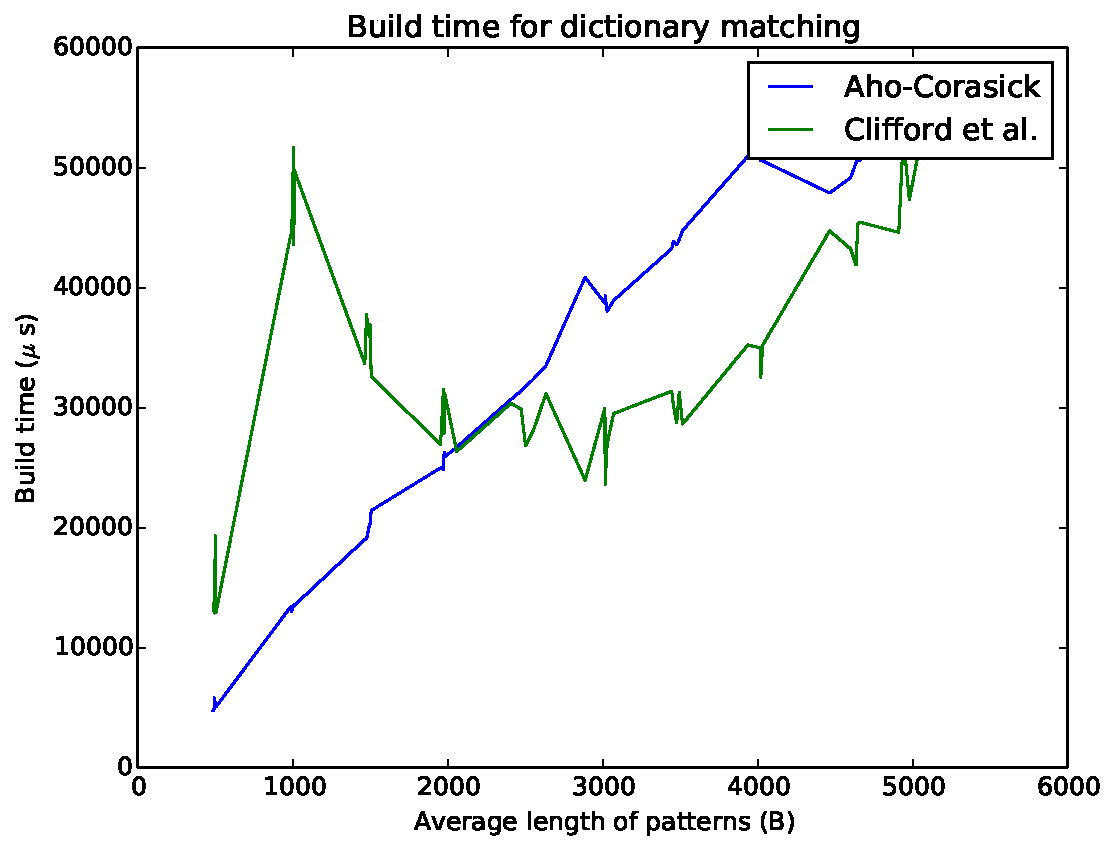
\includegraphics[width=0.5\linewidth]{build_length_1000_10000}\\
  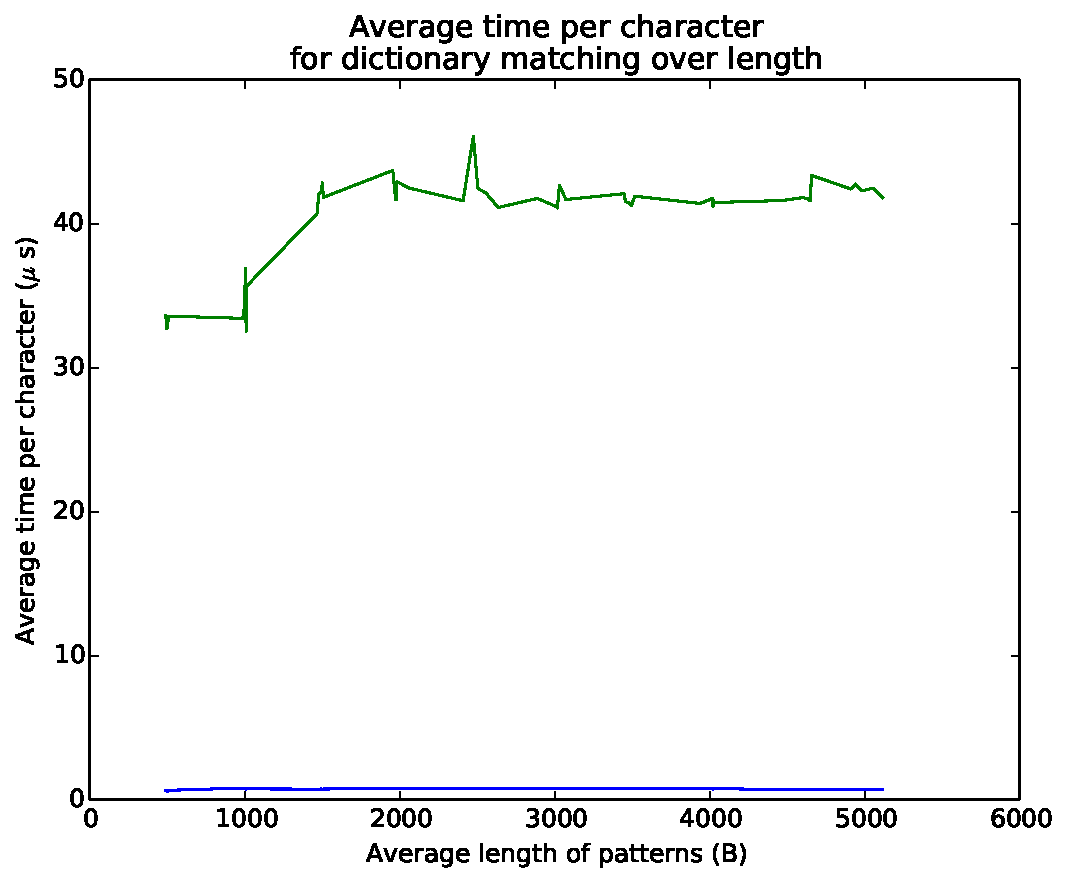
\includegraphics[width=0.5\linewidth]{time_length_1000_10000}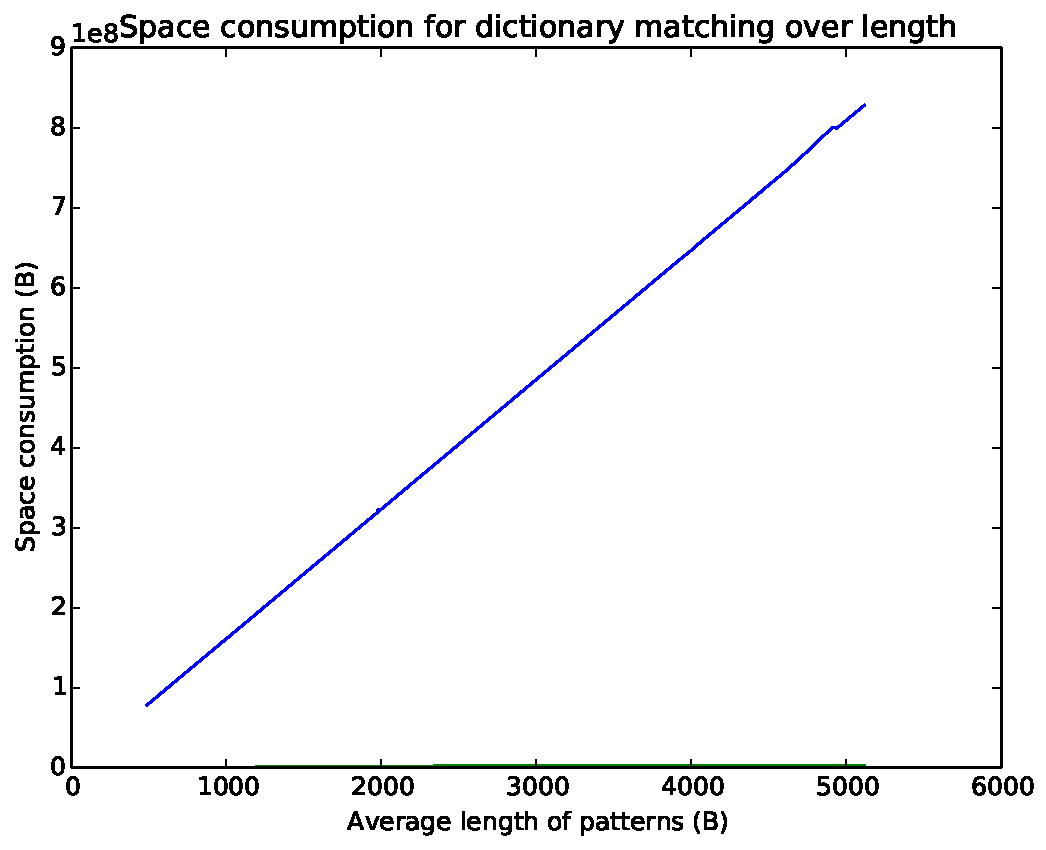
\includegraphics[width=0.5\linewidth]{size_length_1000_10000}
\end{center}
\caption{Build time, run time per character and space for Clifford et al.'s algorithm against Aho-Corasick over the length of the pattern}
\label{fig:long-pattern-results}
\end{figure}

\subsubsection{Build Time}

The first point that can be noticed is the spike for Clifford et al. at roughly 1,000 characters for average pattern length. I was very curious as to why this spike occured, and in particular how it dropped to to nearly half the time for patterns one thousand characters longer and only again started taking that much time to preprocess again at an average length of 5,000 characters. We will look at profiling this case later, but it is worth noting that an average length of 1,000 characters per pattern over a uniform distribution would put the maximum length at roughly 2,000 characters. Since there are 1,000 patterns in total, this would be the upper limit of the case where all patterns are processed using the short patterns case, which would imply that short patterns is a bottleneck with respect to preprocessing time.

The other point that surprised me was how similar these preprocessing times were. Following the preprocessing times from my summer project and how significantly faster KMP was than Breslauer and Galil, I was expecting something similar here. Instead, the algorithm by Clifford et al. in fact took \textit{less} time in most cases. It seems that the more complex state machine required by Aho-Corasick results in a larger overhead than Knuth-Morris-Pratt. I would've liked to have measured this for even longer patterns, due to the fact that the build time of Clifford et al. is getting closer to that of Aho-Corasick by the time the patterns reach an average length of 5000 characters, but this was not possible due to time constraints.

\subsubsection{Run Time per Character}

Another interesting change in time complexity happens at an average pattern length of 1,000 characters for the algorithm by Clifford et al. when it comes to run time per character. But this time it is in the opposite direction, jumping from just under $35\mu s$ to roughly $40\mu s$ between 1,000 and 2,000 long characters for the average pattern length. This seems to imply that, while the short patterns algorithm is a bottleneck for preprocessing, they are actually one of the faster aspects of the algorithm as far as actual processing is concerned.

As far as actual performance is concerned, the Aho-Corasick algorithm is roughly 80 times faster per character than Clifford et al. One point that surprised me is that beyond the increase at the start, we don't see any noticeable increase in time complexity per character as the average length of the patterns increase. This goes against the theoretical analysis, which states that we should see a logarithmic scaling. This would've made for another good reason to test on even longer patterns were time available to do so.

\subsubsection{Size of Data Structure}

Data structure size was a significant surprise to me. I was expecting the size of the data structure to be less -- this is comparing a logarithmic size data structure with a linear size one, after all -- but I was not expecting it on the scale shown in the graphs. To give an idea of how significant this difference is, even on the shorter patterns -- patterns with an average length of 500 characters long -- the data structure for Aho-Corasick was roughly 140 times larger than that of Clifford et al. By the longest average pattern lengths of 5,000 characters, this had grown to approximately 250 times larger.

\subsection{Performance for Shorter Patterns}
\label{ssec:short-pattern-results}

I was originally going to do further testing on higher number of patterns of similar lengths to the ones in Section~\ref{ssec:long-pattern-results}. However, I decided this was of little interest as we already knew what the result would be if we started testing, for example, 2,000 patterns of 5,000 characters each: Aho-Corasick would remain performing better at time complexity while Clifford et al. would perform better at space. As a result, I figured it was more interesting to try shorter patterns, and see if we could decrease the gap in performance between the two algorithms.

These results are shown in Figure~\ref{fig:short-pattern-results}. Each test now conists of 100 patterns, each pattern of lengths uniformly selected as before except the maximum length now ranges from 200 to 1,000 characters. Again, five tests were run for each maximum length.

\begin{figure}[t]
\begin{center}
  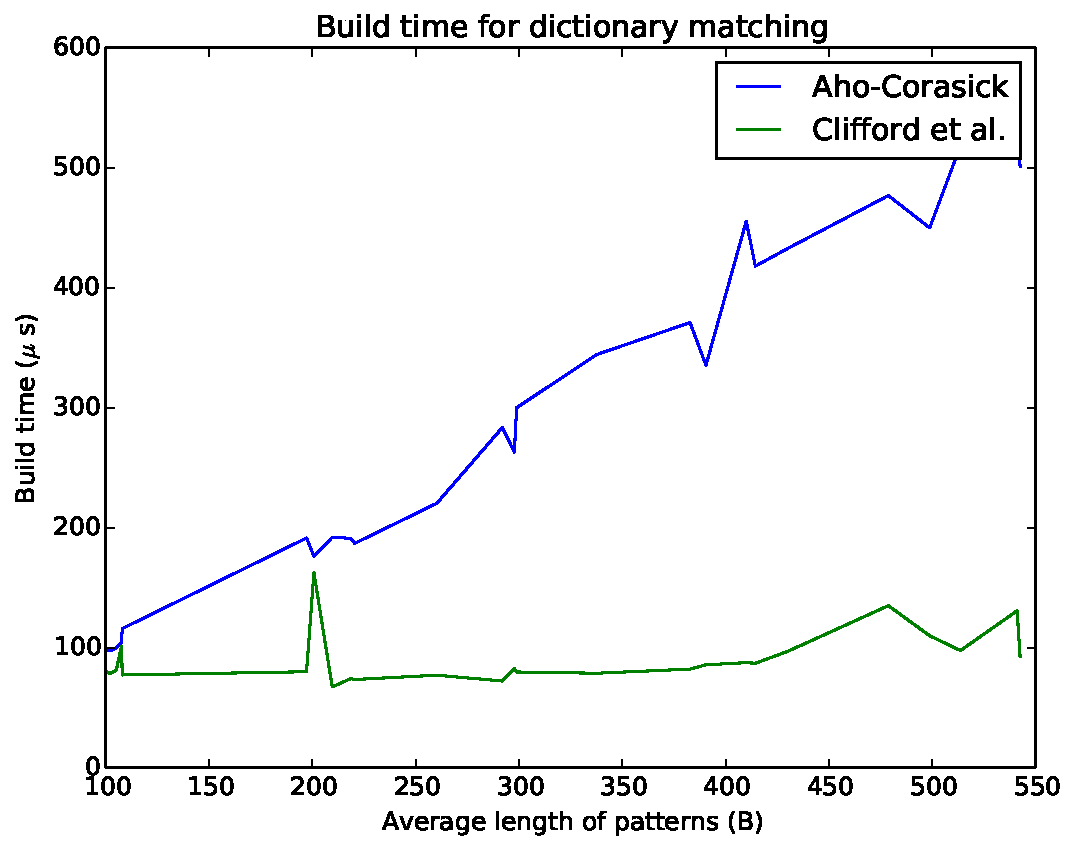
\includegraphics[width=0.5\linewidth]{build_length_200_1000}\\
  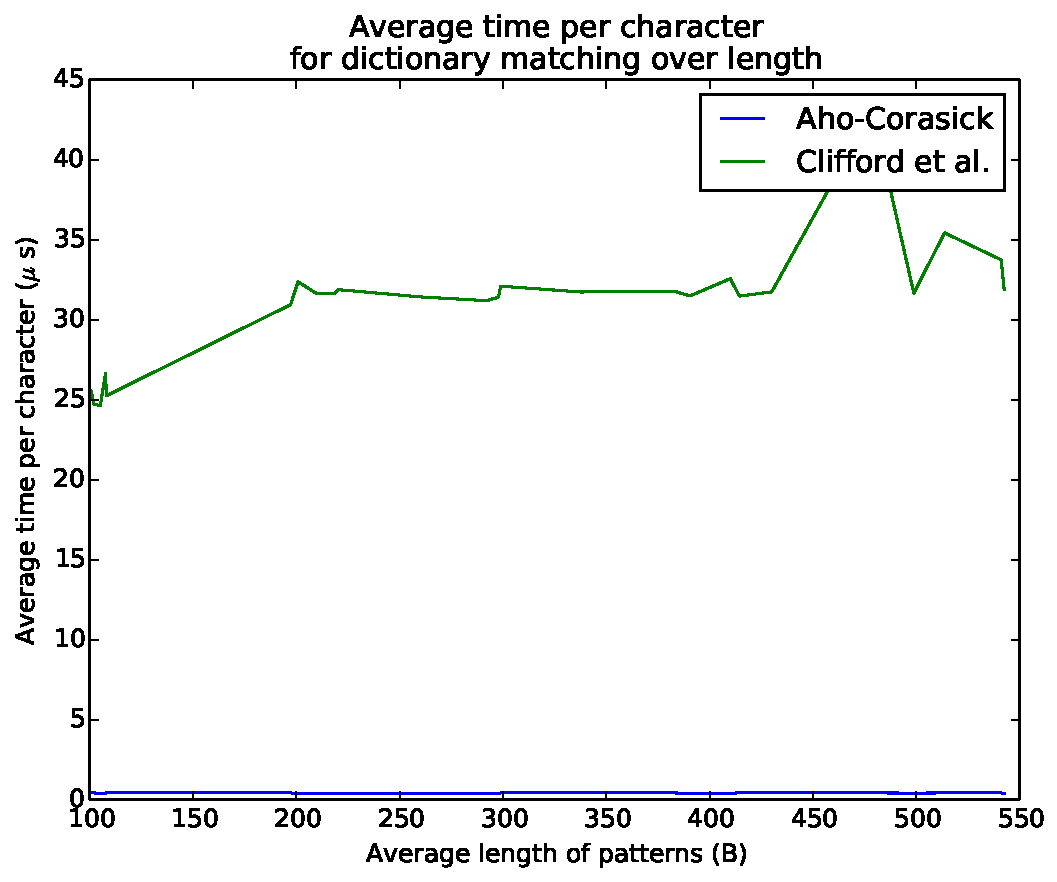
\includegraphics[width=0.5\linewidth]{time_length_200_1000}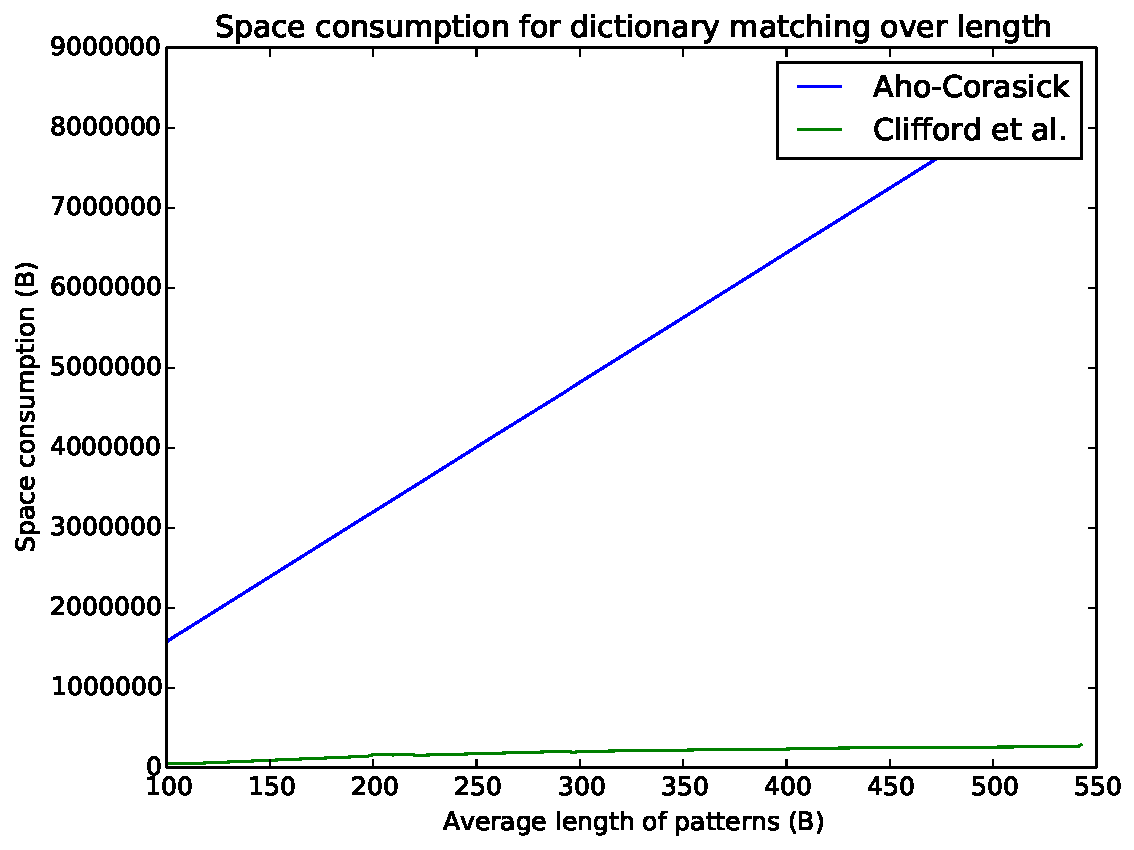
\includegraphics[width=0.5\linewidth]{size_length_200_1000}
\end{center}
\caption{Build time, run time per character and space for Clifford et al.'s algorithm against Aho-Corasick over the length of the pattern}
\label{fig:short-pattern-results}
\end{figure}

\subsubsection{Build Time}

Build time shows similar results as before, though there are some differences. First of all, the spike for cases where all patterns are deemed short is still there, but it is a lot less noticeable. In particular, it has now formed two spikes: One at an average length of 100 characters and another, larger one at 200 characters. This might simply be a granularity issue, and might perhaps be an argument for testing patterns 150, 250 etc. characters long on average, to see if the spike becomes more distinct then.

We can also see the same trend as before in terms of comparing the two algorithms. They start off pretty close when looking at short patterns, but Aho-Corasick then starts taking longer as the patterns grow. From just over 200 characters onwards, the preprocessing time of Clifford et al. is increasing, but a much more gradual rate. There is a bizarre spike at the end of the pattern, however, which will be investigated more when we discuss run time per character.

\subsubsection{Run Time per Character}

Again, we see similar results here as in Section~\ref{ssec:long-pattern-results}. Time taken per character goes up after 200 characters as fewer patterns are deemed short, and that run time is roughly level for the rest of the tests. Overall, the Clifford et al. algorithm takes roughly 80 times longer per character than Aho-Corasick.

One interesting point is that there is a bizarre spike between 450 and 500 characters. We can also notice a spike in the same location for build time. The most likely explanation is that this test is anomalous, potentially caused by a caching issue with GMP or CMPH.

\subsubsection{Size of Data Structure}

For this range of pattern lengths, we are able to see the trend in size for dictionary matching better. In particular, we can see that the case where the patterns are short takes up less space than the long patterns case. It is hard to tell however if this is the result of a constant factor or just due to the fact that the patterns themselves are shorter.

Compared to Aho-Corasick, we still see a saving in space, but the saving is less dramatic. The structure is about 30 times smaller at both the smallest tests -- 100 characters long on average -- and the longest -- 500 characters on average -- but as the algorithms for longer patterns start running at 200 characters on average, this performance drops to twenty times smaller.

\subsection{Performance for More Patterns}
\label{ssec:many-pattern-results}

The next results, shown in Figure~\ref{fig:many-pattern-results}, display the performance or the two algorithms as the number of patterns increases. The lengths of the patterns are randomly selected between 1 and 2000 characters. The number of patterns covered a range between 200 and 1000. For every number of patterns, five tests were run and the performance of these tests were averaged to give these results.

\begin{figure}[t]
\begin{center}
  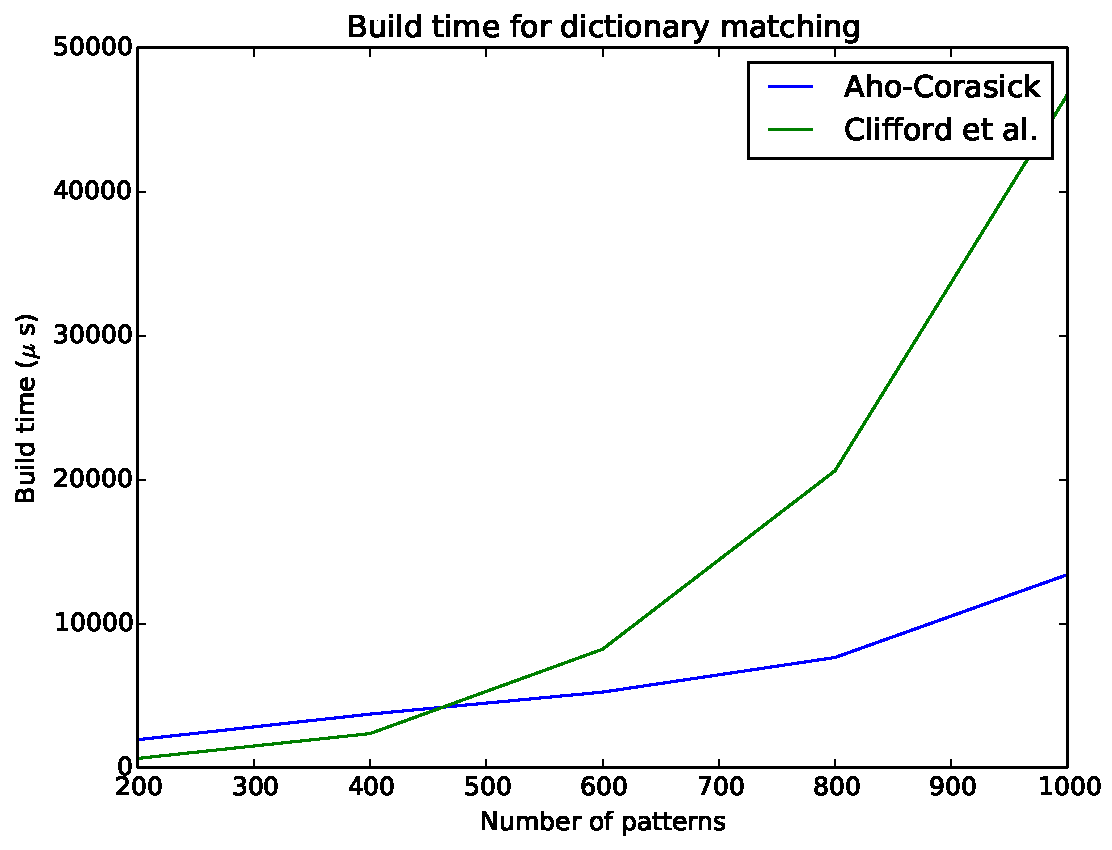
\includegraphics[width=0.5\linewidth]{build_num_200_1000}\\
  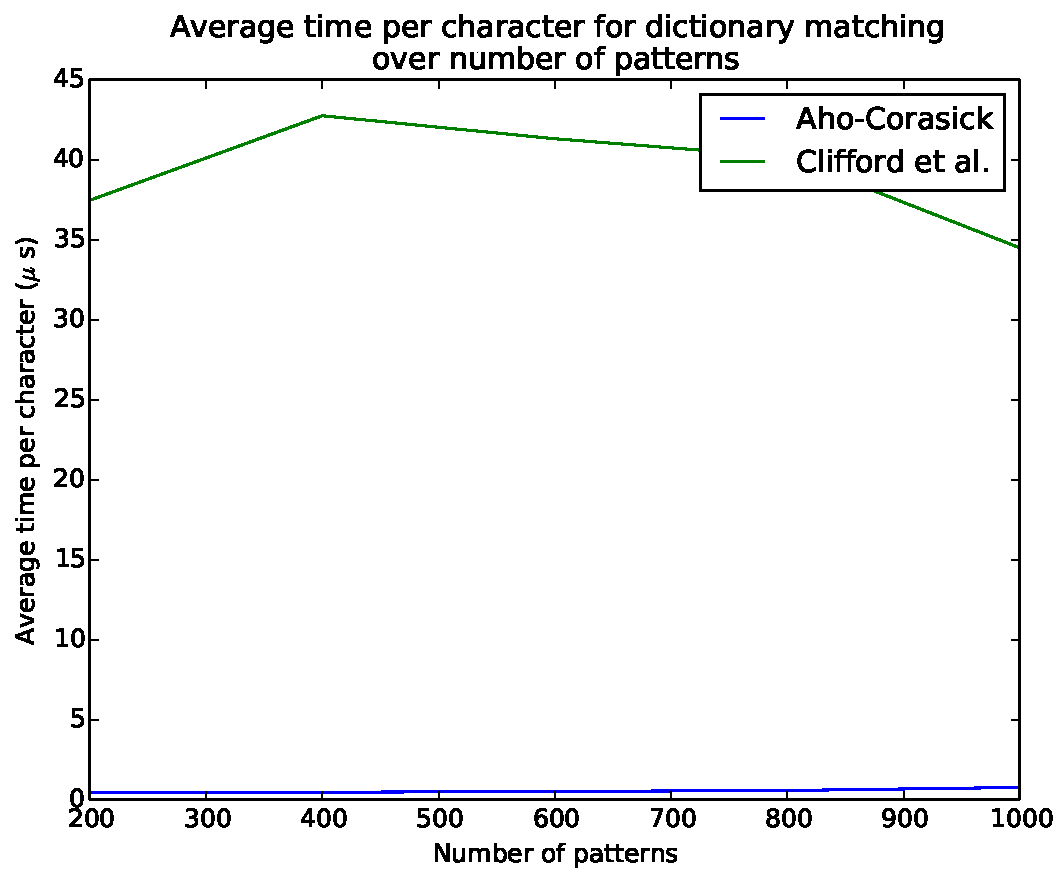
\includegraphics[width=0.5\linewidth]{time_num_200_1000}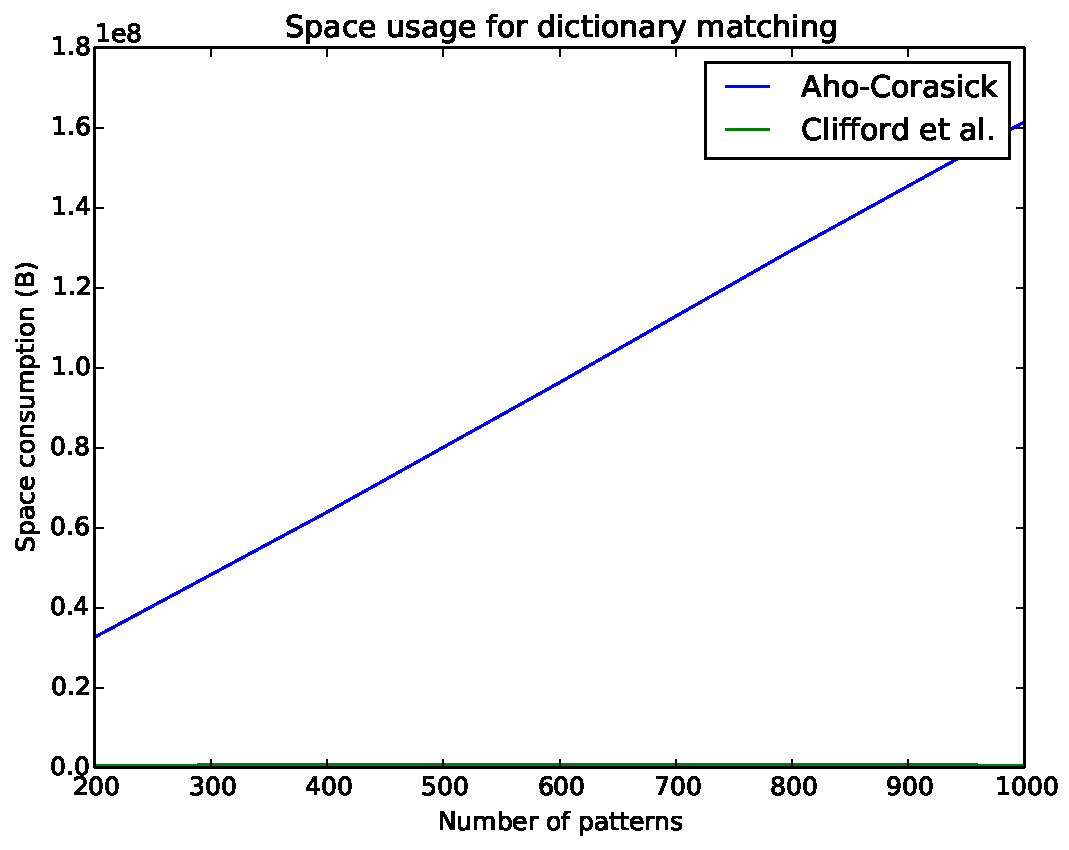
\includegraphics[width=0.5\linewidth]{size_num_200_1000}
\end{center}
\caption{Build time, run time per character and space for Clifford et al.'s algorithm against Aho-Corasick over the number of patterns}
\label{fig:many-pattern-results}
\end{figure}

\subsubsection{Build Time}

Here we have the opposite effect to what we had in Sections~\ref{ssec:long-pattern-results} and \ref{ssec:short-pattern-results}, with the two algorithms taking similar lengths of time as before, yet Clifford et al. taking dramatically longer from about 600 patterns onwards. This adds further confirmation to the claim that short patterns are a bottleneck for preprocessing; since patterns are defined as being short relative to the number of patterns, as we add more patterns to the dictionary yet the length of the patterns on average remains the same, more patterns start being processed by the short patterns algorithm.

\subsubsection{Run Time per Character}

Again, we have the opposite effect to what happened in the previous sections. Clifford et al. started roughly 85 times slower, peaked at 400 patterns when it was roughly 90 times slower, and then started to speed up again until it was just over 40 times slower. This supports the theory that the short patterns algorithm is faster than the long patterns case when it comes to processing time.

\subsubsection{Size of Data Structure}

The size of our data structure is comparable to the graph we saw in Section~\ref{ssec:long-pattern-results}. At 200 patterns, the algorithm by Clifford et al. was roughly 60 times smaller than the data structure for Aho-Corasick. By 600 patterns, when just over half of them on average would be deemed short, Aho-Corasick was roughly 95 times larger, and at 1000 patterns it became 260 times larger.

\subsection{Performance as $\alpha$ Increases}

At the end of Section~\ref{sec:kr-fingerprints}, when we discuss the probability of a collision in the fingerprints, we mention that the Karp-Rabin fingerprints take a precision value $\alpha$ during construction. A larger value for $\alpha$ results in a larger prime, as $p \in O(n^{2 + \alpha})$. If we were using native 32 or 64 bit integers, then this would have no effect on performance. But because we are using multiple precision integers, this can affect all aspects of performance measured, as preprocessing time, run time and size all depend on the respective performance of the individual fingerprints being constant.

To analyse this, we measured the performance of the Clifford et al. algorithm with values for $\alpha$ ranging between 0 and 5. For each value of alpha, five tests were run and the average performance of these results were taken. Each test consisted of 100 patterns varying between 1 and 400 characters long. The results of these tests are shown in Figure~\ref{fig:alpha-results}.

\begin{figure}[t]
\begin{center}
  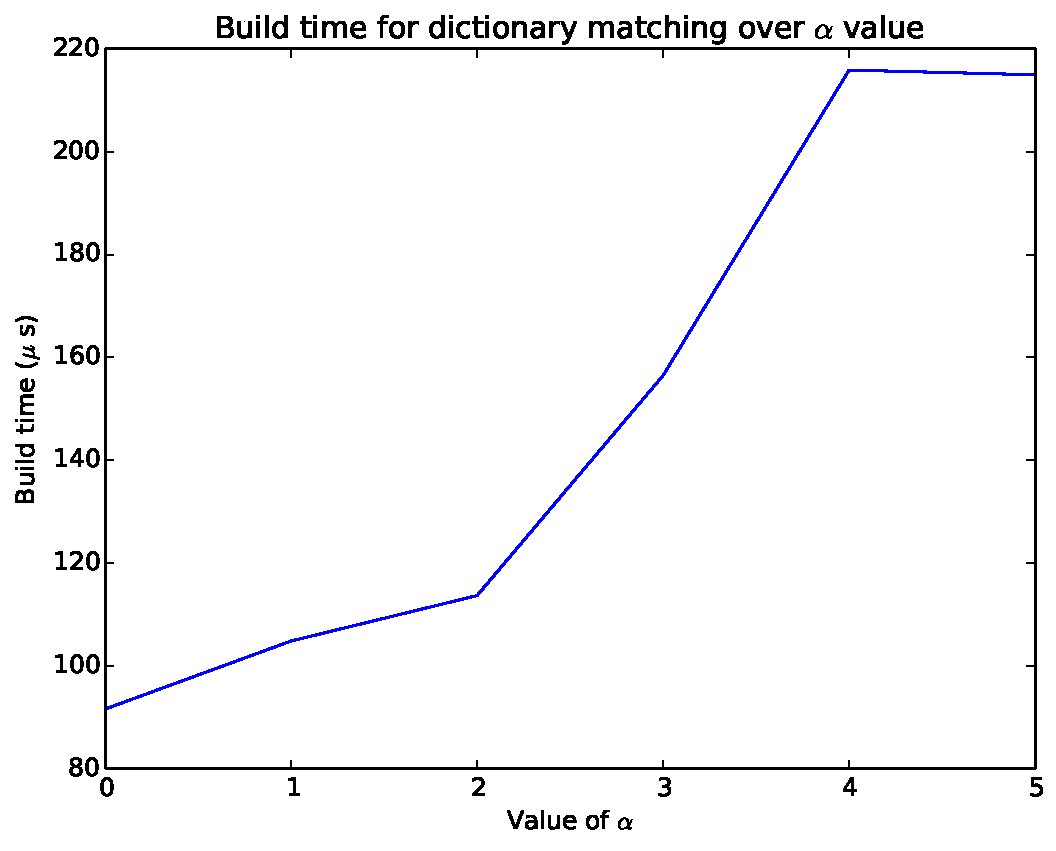
\includegraphics[width=0.5\linewidth]{build_alpha}\\
  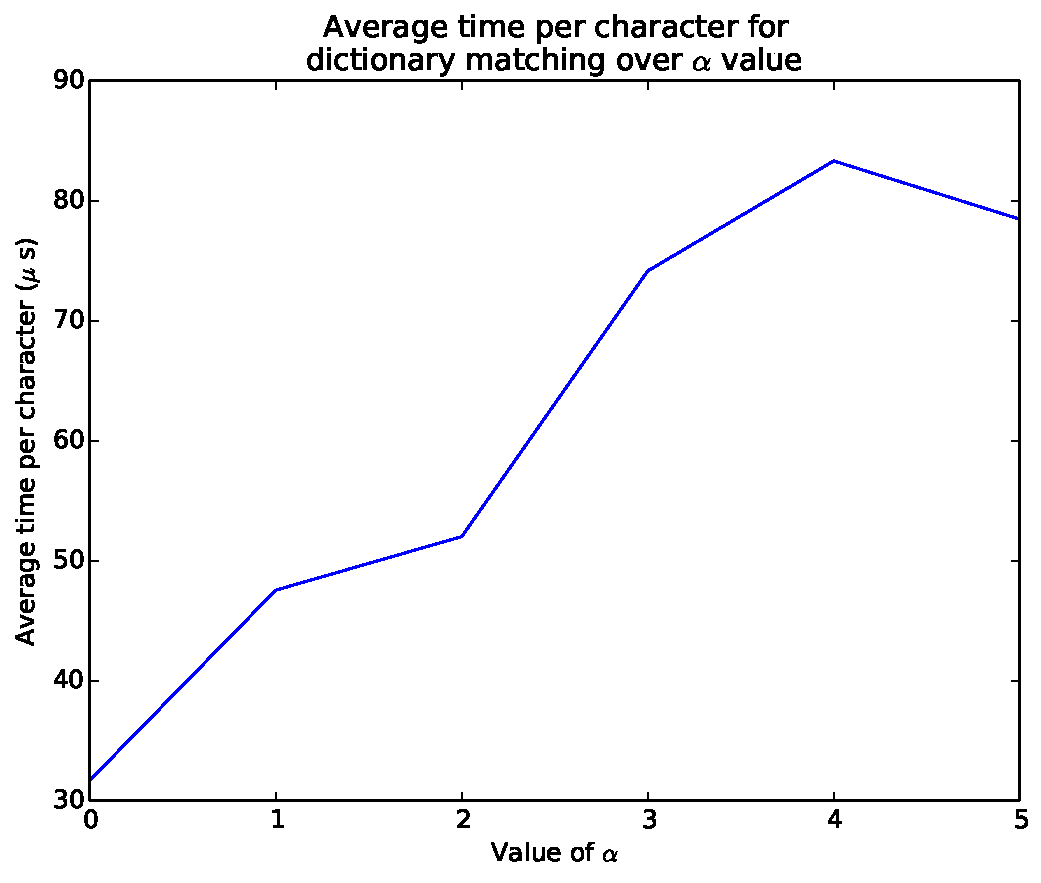
\includegraphics[width=0.5\linewidth]{time_alpha}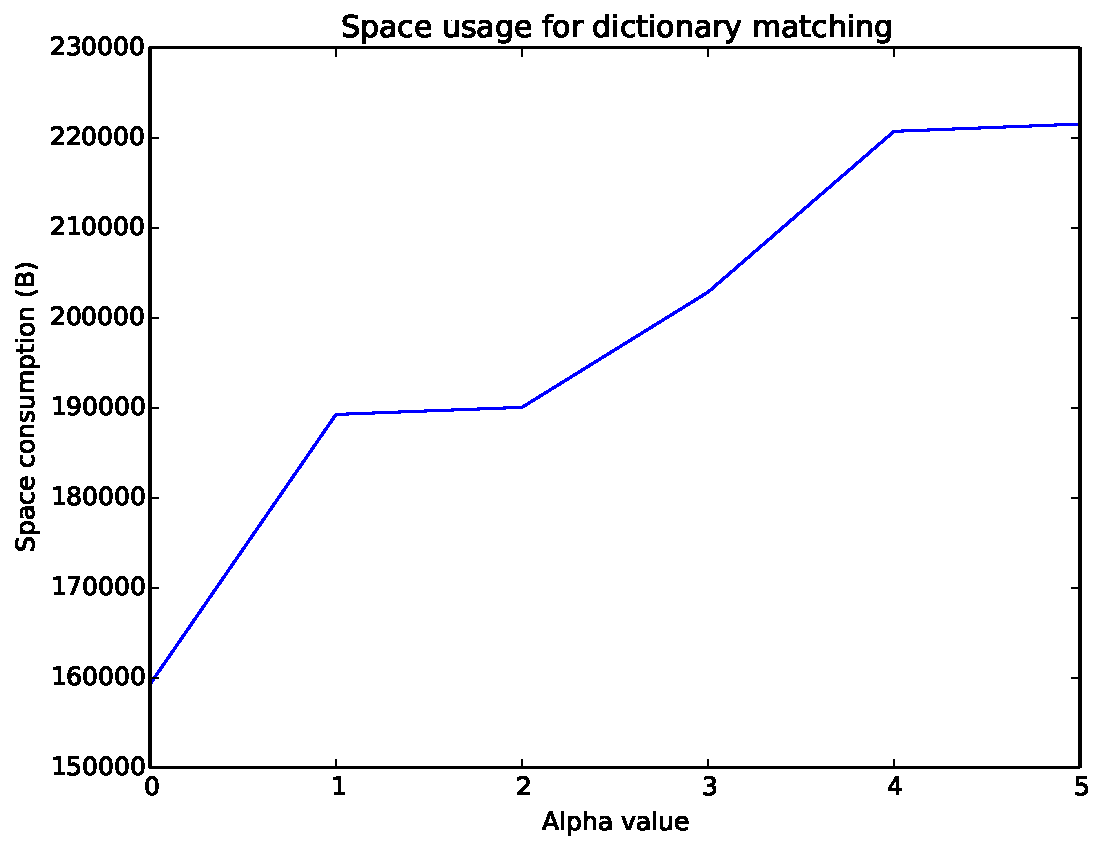
\includegraphics[width=0.5\linewidth]{size_alpha}
\end{center}
\caption{Build time, run time per character and space for Clifford et al.'s algorithm as $\alpha$ increases}
\label{fig:alpha-results}
\end{figure}

Intuitively, we would expect the performance to increase linearly as $\alpha$ increases. This is because all fingerprints are bounded by $p$, which can be represented in $\log p$ limbs, and $p$ increases exponentially in terms of $\alpha$. Thus we would expect as $\alpha$ increases, the number limbs required to represent $p$ would be $O(\log n^{2 + \alpha}) \in O((2 + \alpha)\log n) \in O(\alpha)$ due to $n$ being a constant.

We can see this change, but the actual scaling is more complex: The performance for all three traits grows at steep rates for $\alpha$ values from 0 to 1 and 2 to 4, before becoming shallower at ranges such as 1-2 and 4-5. This is due to how GMP itself allocates and handles space for limbs. It overcompensates, allocating more limbs than are needed at points to avoid having to do more reallocations later on.

\subsection{Space Consumption for Each Case}

We will to some extent investigate the time taken for each case in Section~\ref{sec:profile-results}, but for now we can look at the space consumption for each of the cases in Clifford et al.'s algorithm. These results are shown in Figure~\ref{fig:case-results}.

One caveat to bear in mind is that the main data structure for this implementation is the structure for long algorithms, and thus contains various shared fingerprints -- including the shared buffer of the last $2k$ fingerprints of the text, the fingerprint of the whole text and a fingerprint just for temporary values -- and thus is not entirely representative of the space consumption of the algorithm alone. The tests that this might affect are as the number of patterns or $\alpha$ increase, as the size of the shared items only scale in terms of $k$ and $\alpha$.

\begin{figure}[t]
\begin{center}
  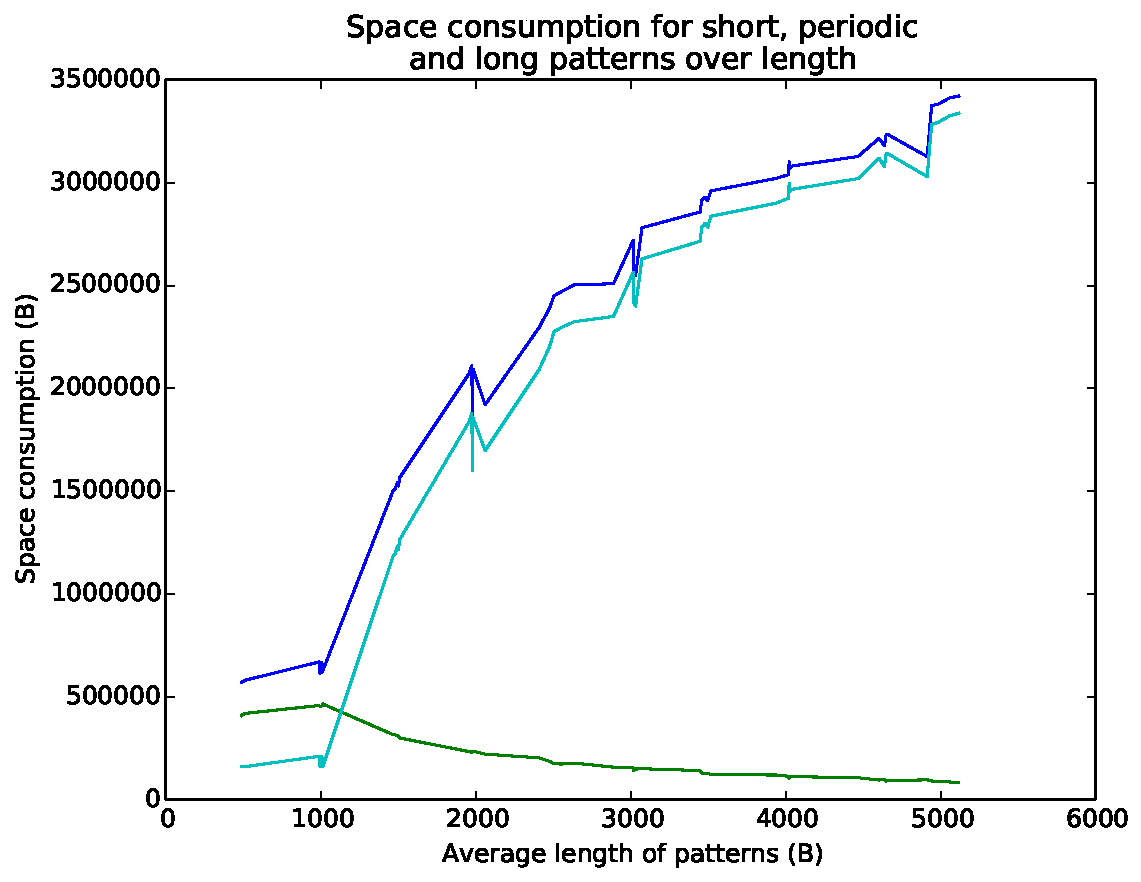
\includegraphics[width=0.5\linewidth]{part_size_length_1000_10000}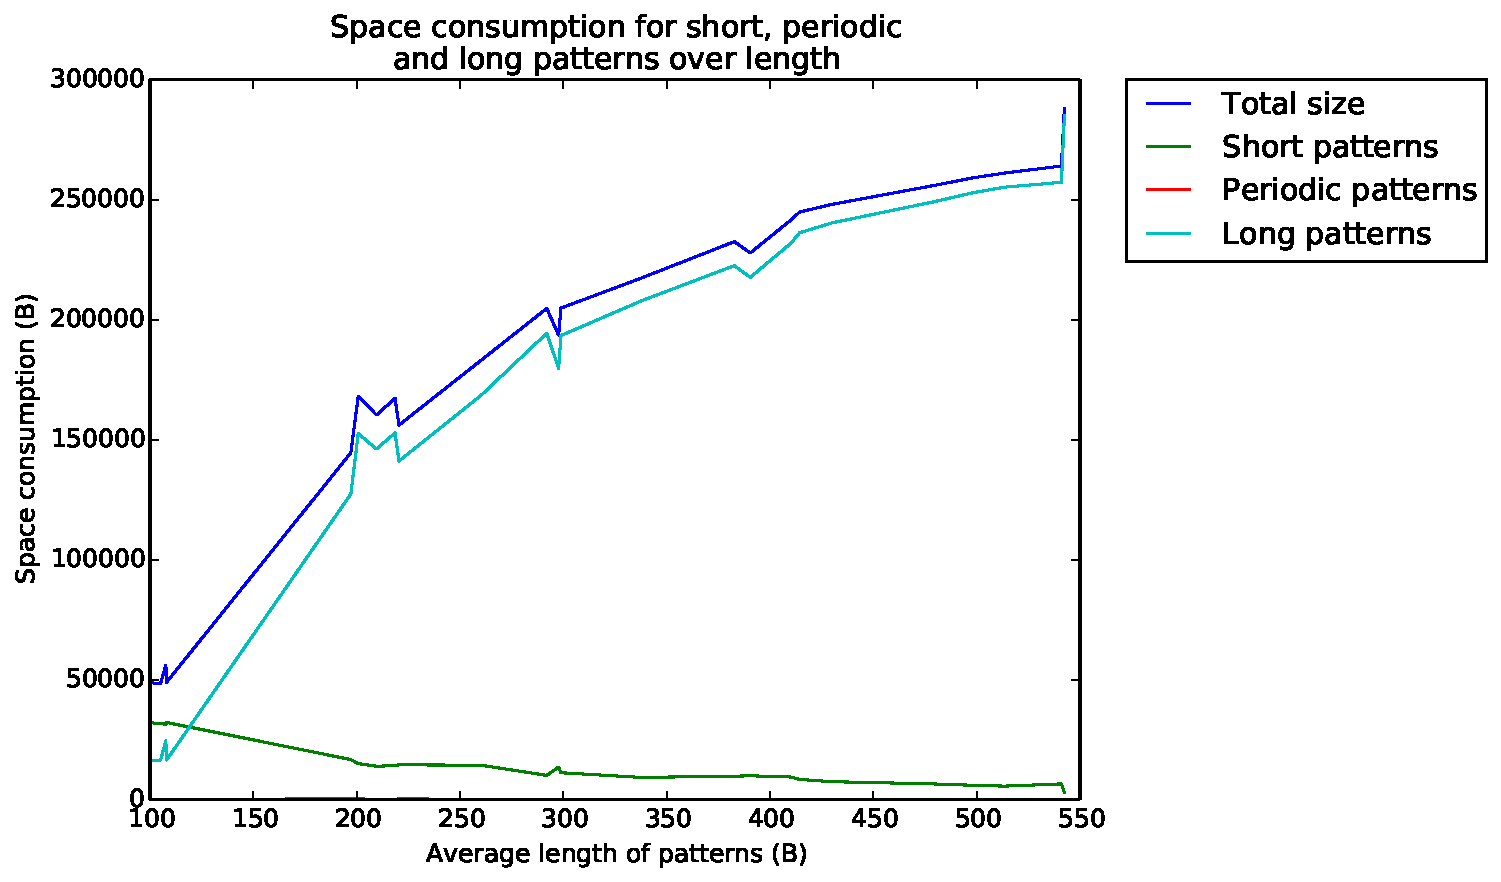
\includegraphics[width=0.5\linewidth]{part_size_length_200_1000}
  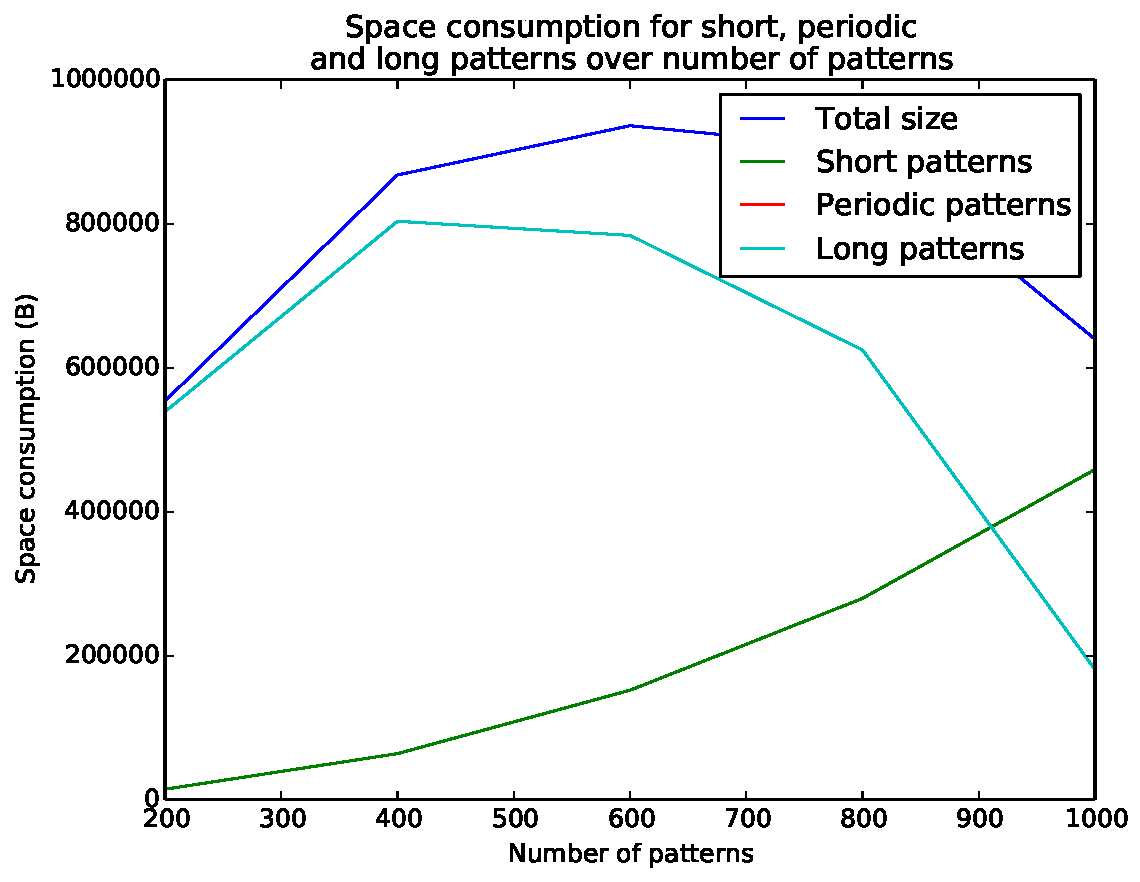
\includegraphics[width=0.5\linewidth]{part_size_num_200_1000}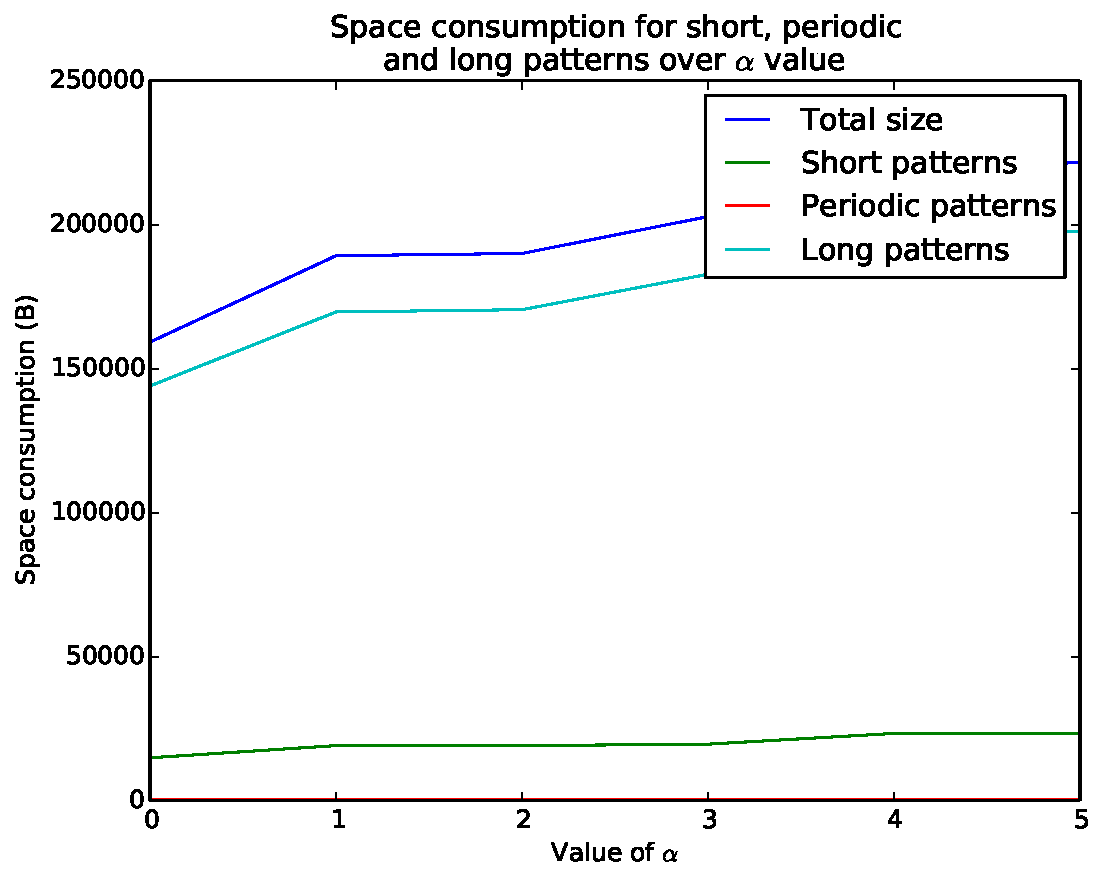
\includegraphics[width=0.5\linewidth]{part_size_alpha}
\end{center}
\caption{Size of short, periodic and long algorithms for dictionary matching}
\label{fig:case-results}
\end{figure}

The first point that can be seen is that the size consumption of long patterns with short periods is too small to even register on these graphs. Unfortunately, I doubt this is due to the algorithm for long patterns with short periods being very efficient in terms of memory. The more likely scenario is that the patterns used to test this work just did not hit this case frequently. This is understandable; even on data as repetitive as DNA we are very unlikely to have genomes repeating enough to be longer than $2k$ while also having a period of at most $k$ characters long. This is especially true when $k$ is in the hundreds or even thousands.

We can also tell from these measurements that, even taking into account the caveat at the start of this section, the main space consumption is the algorithm for long patterns. The long patterns with short periods algorithm has barely any effect due to the reasons stated above, and the short patterns algorithm only becomes the bottleneck in the tests when all patterns are deemed short. In any other case, the total size roughly follows the same curve as the size of the data structure for patterns with long periods.

As for $\alpha$ values, the sizes do scale as expected, but they all follow the same general trends for scaling, merely within a constant factor of each other. This is unsurprising; we do not classify whether a pattern is long, periodic or short based on the value of $\alpha$. Thus a larger $\alpha$ will not affect the number of patterns assigned to each algorithm, which is the main reason for the algorithms scaling differently in the other graphs.

\subsection{Frequency of False Results}

The final aspect I wanted to investigate was how much the two algorithms disagreed in terms of their results. There are two reasons for this analysis:

\begin{enumerate}
  \item I wanted to see how much the inaccuracy in fingerprints and the introduction of randomness affected the results.
  \item I wanted to see how frequently the edge cases were hit.
\end{enumerate}

For this, I measured the number of matches from both algorithms when applying the tests over average pattern lengths and number of patterns described in Sections~\ref{ssec:long-pattern-results}, \ref{ssec:short-pattern-results} and \ref{ssec:many-pattern-results} and computed the difference. Assuming Aho-Corasick ran correctly, I took the number of matches from Aho-Corasick and subtracted the number of matches from Clifford et al. and represented the difference as a percentage of the number of matches made by Aho-Corasick. For number of patterns, I did the same as before and took the average for each test. The results can be seen in Figure~\ref{fig:diff-results}.

\begin{figure}[t]
\begin{center}
  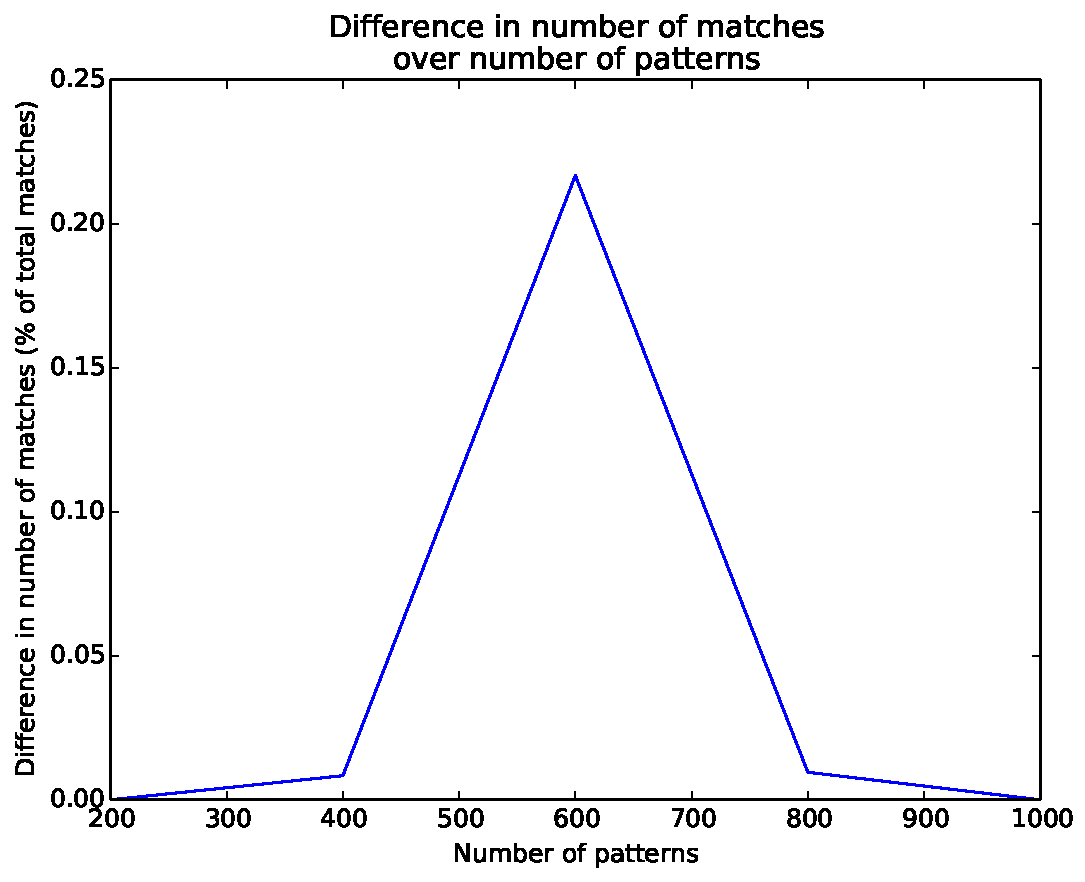
\includegraphics[width=0.5\linewidth]{diff_num_200_1000}\\
  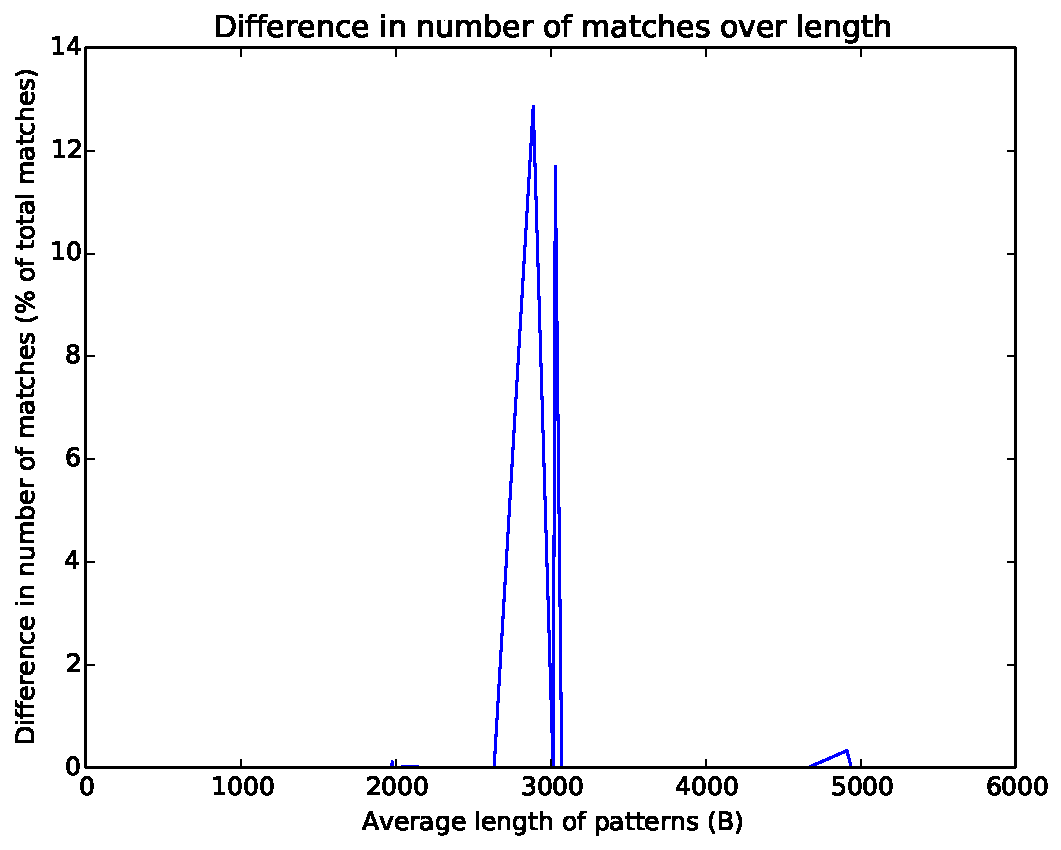
\includegraphics[width=0.5\linewidth]{diff_length_1000_10000}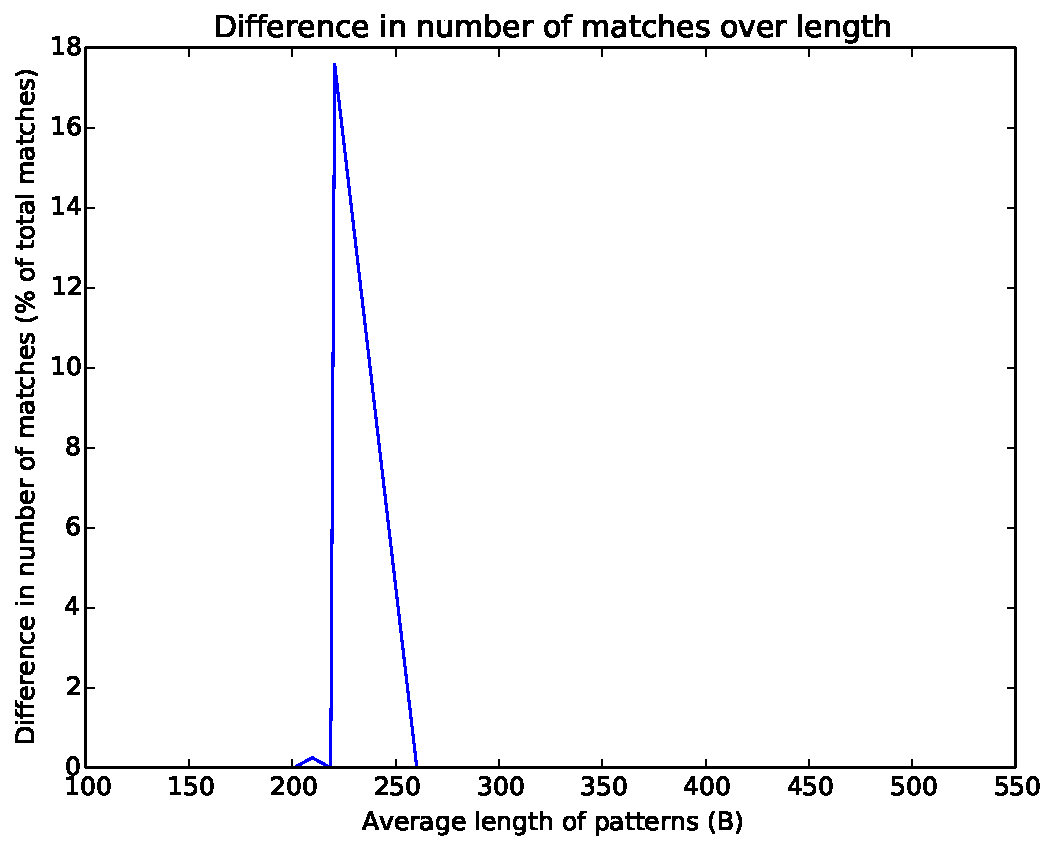
\includegraphics[width=0.5\linewidth]{diff_length_200_1000}
\end{center}
\caption{Difference in number of matches between Aho-Corasick and Cliffort et al. implementation}
\label{fig:diff-results}
\end{figure}

It is unlikely that these differences have occurred due to collisions in the fingerprints; having run some of these tests multiple times, the number of matches has remained consistent throughout. This means that the more likely scenario is the Clifford et al. algorithm hitting the edge cases.

We can observe that for the graphs where the patterns are increasing, the peaks are where the average pattern length is roughly 2-3 times larger than the number of patterns. We can analyse this with the definition in Section~\ref{ssec:impl-edge-case} in mind. If the average pattern length is 3,000 characters for 1,000 patterns, then the average length of the prefixes $Q_i$ is 2,000 characters, and thus the length processed by power of two matching is 1,024 characters. At this point, the start and end of the pattern only need a few characters in common to have a period shorter than the number of patterns.

This doesn't hold however with the number of misses over number of patterns. Otherwise, the peak would be before 600 patterns, as the average length of each pattern is 1,000 characters. A number of potential reasons could be behind this, from our scale being too granular -- we don't measure 300 patterns, which would roughly be the peak in this case -- to our averages cancelling out.

The final point to emphasise is that, while these can be pretty severe when looking at the individual tests -- the worst case was nearly 18\% of all matches missing -- a high degree of this is bad luck with the randomly generated patterns. We can see from the graphs that the peaks are very steep, which implies that while some dictionaries were poor, others matched near-perfectly. When these tests are averaged out, as they are for the number of patterns, the number of misses drops significantly, peaking at less than a quarter of total matches. Even in the cases where mistakes have occurred, it is likely that these were a frequent minority of problematic patterns rather than most patterns hitting the edge case.

\subsection{Profiling Results}
\label{sec:profile-results}

In order to find bottlenecks, I ran the Clifford et al. algorithm on three test cases:

\begin{itemize}
  \item 1000 patterns up to 2,000 characters long, to see why there is such a big spike in preprocessing time at this point.
  \item 1000 patterns up to 4,000 characters long, to see how the algorithm performs when roughly half the patterns are short and half are long.
  \item 1000 patterns up to 10,000 characters long, to see how the algorithm performs when few of the patterns are short.
\end{itemize}

For both tests, the first point I saw was that the main bottleneck, with roughly 60\% of the total (preprocessing and running) time was actually the function for checking if two fingerprints are equal. The reason is not because the function is a slow one -- on the contrary, it is one of the fastest functions in the entire source code as simply three calls to \texttt{mpz\_equals} -- but it is called so frequently that even if it takes virtually no time to execute, that time still adds up overall. To give an idea of how many times it is called, for the first of the two tests listed above on 50MB of text, it was called nearly 680 million times on the actual processing alone. It was called another 17 million times in preprocessing, resulting in just over 696 million calls to the function in total. The same story is true for the second case, where it was called a total of 825 million times.

This was also the reason why preprocessing for short pattern dictionary matching was so slow. When I first saw the spikes, I thought it would be because of the suffix function $\mathcal{S}$, which uses na\"{i}ve string matching to check if one of the $k$ patterns is the suffix of a string. But this actually runs relatively fast due to the choice of data; it is unlikely for two randomly selected patterns to match for a long time. The actual reason for the spike was because roughly two thirds of that time was spent checking with linear search if a fingerprint was already going to be added into the hash table. Each time we checked this, it would take $O(k\log m)$ time to do so, resulting in an overall performance of $O((k\log m)^2)$ for preprocessing.

As far as calling the equals function for fingerprints, the main cause is the short patterns algorithm. In the second profiling case, 80\% of calls were made by the short patterns algorithm during processing. That's 666 million calls from this one function, or roughly 12.7 calls for each character of the text, just from the short pattern case. This also results in the short patterns case taking up 23\% of the total running time for the whole test program.

For patterns with long periods, there are two main bottlenecks. The first is shifting patterns. Although \texttt{gprof} itself is not offering much information on where the slowdown is, intuition points towards the Red-Black Tree. In particular, deleting items from the RBT is called frequently and might reasonably cause a drop in performance due to both the heavy reliance on the heap and the $O(\log k)$ bound itself. Unfortunately, there is little further analysis we can do using \texttt{gprof} to verify this. This is because \texttt{gprof} is very poor when it comes to mutual recursion \cite{SPE:SPE562}, which is what you have in the case of RBT source code: \texttt{delete\_case1} calls \texttt{delete\_case2} which calls \texttt{delete\_case3} which might call \texttt{delete\_case1}. The other bottleneck for patterns with long periods is, once again, checking if fingerprints are equal.

There was something curious however about the second and third tests. The main bottleneck was short pattern dictionary matching, followed by checking if two fingerprints were equal. What particularly surprised me was that short dictionary matching was now making \textit{more} calls to the function for checking if fingerprints matched, not fewer. But surely if a pattern matching algorithm has fewer patterns then it should result in fewer function calls? And if short patterns is the bottleneck, why is it so much faster when all patterns are short?

This confused me, but then I realised what was actually happening to make short patterns such a bottleneck. The short patterns algorithm takes $O(\log k)$ time in the case where there are \textit{no matches} at a given index, as this is the point when it needs to perform a full binary search. As patterns become longer, fewer patterns are deemed short, and thus there are fewer patterns for this algorithm to match. Because all the patterns generated were substrings of the text, if there are fewer patterns for an algorithm to process then it is less likely to find a match. As a result, when the patterns grew longer, there were fewer matches for short patterns, which meant that worst case time complexity was happening more frequently for this case.

\section{Proposed Improvements}

As can be seen from the past few pages of evaluation, there is a lot that this implementation does well. In particular, the data structure size is a significant advantage over Aho-Corasick. However, there are still a number of points where we can see improvements, in both theory and practice, which can lead to an even better performing algorithm. While none of these were implemented due to lack of time, they can provide some discussion on what choices might have been better for this project, as well as directions for future work.

\subsection{Reducing Bottlenecks}
\label{sec:reduce-bottle}

Following on from Section~\ref{sec:profile-results}, it only makes sense to discuss the bottlenecks discovered there first of all.

A good place to start in this discussion is, obviously, the major bottleneck found from profiling: Checking if fingerprints are equal. Unfortunately, there are very few things we can do to speed up the run time of \texttt{mpz\_equals} itself, but there is a simple way of cutting down the number of times we need to call it. Instead of using \texttt{mpz\_equals} to compare \texttt{r\_k} and \texttt{r\_mk} to test if the strings are the same length, we could simply add a 32-bit integer to the fingerprint data structure to represent the actual length of the underlying strings and then just compare these integers. This offers the benefit of native integer comparison being significantly faster on a CPU than multiple precision integer comparison. We also now get the added bonus that the probability of different length strings colliding is the same as strings which are the same length, assuming that we are not comparing patterns which are individually gigabytes long. There is an extra four bytes per fingerprint, but particularly for long patterns this cost is affordable. We will look at another potential improvement in Section~\ref{ssec:do-we-need-mpa}, but beyond these two the only other optimisation we can really make to this bottleneck is to reduce the number of calls to this function.

When it comes to checking for duplicate fingerprints during preprocessing, we can reduce the number of equality checks by using a binary search tree instead of linear search. In the case of short pattern matching, this alone can reduce the build time from $O((k\log k)^2)$ to $O(k\log k\log(k\log k))$. We already have a function for comparing fingerprints from Section~\ref{ssec:static-hash-fail}, but this function assumes that the underlying strings are the same length, which we do not have in the short patterns case. This can be rectified by adding an additional integer for string length, as suggested in the above paragraph: We first compare the lengths, and if they are the same length then we compare the fingerprints.

As for the other, not as significant bottleneck from long patterns, shifting the rows, we can potentially make some improvements in this area as well. If the bottleneck is the tree, then we could try replacing the tree with a dynamic hash table, such as lhash\cite{website:openssl-lhash}. Hash tables can achieve better average or even worst case run times than binary search trees, but might have an overhead in space consumption. With lhash in particular, measuring space is difficult, but still possible by using lh\_stats\cite{website:openssl-lhstats}. The other potential slowdown is the fingerprint operations such as concatenation. We will see how we might be able to speed these up in the next few sections.

\subsection{Improving Fingerprint Performance in General}

While Sections~\ref{ssec:pick-p}, \ref{ssec:p-size} and \ref{ssec:do-we-need-mpa} look at methods related to how we select our prime number $p$ for optimising purposes, this section will look at two general ways of speeding up the performance of fingerprint operations. In particular, there are two broad ways we will look at optimising the algorithm.

The first is a theoretical proposal. We can see that this scheme uses a lot of modular multiplication operations. More importantly, all of these operations have the same modulus $p$. Intuitively, this makes this case a strong contender for Montgomery multiplication \cite{montgomery:multiplication}. Montgomery multiplication works by representing each symbol $a$ as $a\rho \mod p$, where $\rho$ is the smallest number that satisfies $\rho = b^i > p$, where $b$ is the size of each limb in bits and $i$ is an integer. Montgomery multiplication means that, given two integers $a\rho\mod p, b\rho\mod p$, we can compute and return $ab\rho\mod p$. More importantly, we can achieve this without any division, which modulo operations (including GMP) typically rely on. The cost of this is that as each character is processed, we need to convert that character into its Montgomery representation.

One problem with this is that we are doing more than simply modular multiplication: We are also doing addition modulo $p$. Thankfully however, we can see that addition of Montgomery representations works as well from the following fingerprint for a string $S$ where all characters are in Montgomery representation:

$$s_0r^0\rho + s_1r^1\rho + ... + s_lr^l\rho = (s_0r^0 + s_1r^1 + ... + s_lr^l)\rho = \phi(S)\rho \mod p$$

Thus we can conclude that the modular addition of the Montgomery representation of terms yields the Montgomery representation of their sum.

The other general speedup is an applied one. Throughout this work, I have stuck to using the high-level GMP integer functions for addition, subtraction, multiplication and modulo operations. However, all of these operations also have low level equivalents, with all bar modulo written in assembly languages. The disadvatage is manageability, particularly since these functions require specifying the number of limbs to write. But since all operations are modulo $p$, this number is already known. We can also use the function \texttt{mpz\_init2} to allocate enough limbs to every fingerprint for any possible value, as the low level functions do no memory reallocation themselves.

\subsection{Picking $p$ More Carefully}
\label{ssec:pick-p}

Another option as an alternative to Montgomery multiplication is to use Mersenne primes. Mersenne primes are prime numbers of the form $2^p - 1$. Mersenne primes are significantly less frequent than ordinary prime numbers, but are extremely beneficial for modular arithmetic. This is because in binary they are simply a string of 1s, so modulo operations can simply be evaluated as a bitwise AND. This is much more efficient than Montgomery reduction, but comes at the cost that multiple precision addition and multiplication might be more expensive due to the larger primes.

An extra benefit of Mersenne primes is that we do not need to generate and test them ourselves. This is because the hard work is done for us by the Great Internet Mersenne Prime Search\cite{website:gimps-known}. This website features the 44 definite smallest Mersenne primes, which range from 3 to $2^{32,582,657}-1$. A simple linear search would suffice to find the first prime from the range that is longer than $O(n^{2 + \alpha})$, and we are extremely unlikely to want a text length and accuracy level high enough to require a prime anywhere near this maximum.

\subsection{How Large Must $p$ be?}
\label{ssec:p-size}

Throughout this project, $p$ was selected to be the first prime larger than $n^{2 + \alpha}$, which results in the probability of a collision being $\frac{1}{n^{1 + \alpha}}$ as long at the lengths of the two strings $l \leq n$. However, this probability is not entirely necessary; we know the strings have to be shorter than, $n$, as the strings must be shorter than the text. The longest strings we ever test in our implementation are $\max(m, k)$ characters long. In fact, if we follow the suggested change to fingerprint equality mentioned in Section~\ref{sec:reduce-bottle}, then we will only compare the fingerprints of strings which are at most $m$ characters long.

So how large does $p$ need to be? At the very least, we want $p \in O(m^2)$, in order for the above probabilities to hold. We might also want to include $n$ as a factor towards calculating $p$, given that even if we were to use a hypothetical constant time algorithm we would still need to make at least $n$ tests for equality. But $n$ probably does not need to be as big a factor in determining $p$ as it currently is; throughout all of my testing the only collisions I was ever made aware of where cases when the strings were of different lengths, which can then be modified as explained in Section~\ref{sec:reduce-bottle}.

\subsection{Do We Really Need Multiple Precision Arithmetic?}
\label{ssec:do-we-need-mpa}

This final section on speeding up the fingerprint operations builds on Sections~\ref{ssec:pick-p} and \ref{ssec:p-size}. As stated in Section~\ref{sssec:kr-implementation}, there are two significant advantages for using GMP. But these advantages don't hold as much water as initially thought:

\begin{itemize}
  \item Arbitrary precision might matter following the current way that $p$ is defined, but if we were to modify this definition as suggested in Section~\ref{ssec:p-size}, then we probably don't need any integers larger than 64 bits. Even if we were to keep $p$ under the same definition, we can process just under four gigabytes of text just by using 64-bit integers, as $(4 \cdot 2^{30})^2 = 2^{64}$
  \item Fast prime calculation would certainly not matter if we were to use the list of Mersenne primes explained in Section~\ref{ssec:pick-p}, or even if we just implement the prime testing algorithm ourselves.
\end{itemize}

Plus, 64-bit numbers are both faster and more efficient due to their native implementation, and 64-bit architectures themselves are becoming more widespread. So it is worth testing on fixed-size integers as well to see how much practical performance improves from it.

\subsection{Deamortisating the Algorithm}
\label{ssec:deamortise}

As mentioned in Section~\ref{ssec:static-hash-fail} the reason for the amortised time complexity is due to how we insert items into and destroying the Red-Black Tree.

In order to deamortise inserting items into the RBT, we need two counters: One to keep track of the current prefix being checked and another to keep track of the next suffix that needs to be inserted into the tree. For each index of the text, we perform two steps. A step is either inserting another suffix into the RBT, or checking if the text matches and prefix and if so inserting the first suffix for that prefix into the tree. Because there are only $k$ patterns, we can process all steps in $\frac{k}{2}$ characters as before.

To deamortise destroying the tree, this can be achieved by storing pointers to the next non-empty tree to be destroyed in a queue. At each index, two nodes from the tree at the head of the queue are removed. If the tree at the head of the queue only contained two nodes, it is now empty and this destroyed. If it contained one node, then it is destroyed and another is removed from the next tree in the queue.

\subsection{Towards Sublinear Working Space}

There are two points that prevent us from looking at sublinear working space in the streaming model, both of which are to do with preprocessing. We will investigate both in turn, and provide a compromise where it is possible to solve both if we can view the patterns multiple times.

The first problem is computing the periods. It is possible to compute the periods for each pattern in a stream\cite{ergun:sublinear-period} using $O(k\log m)$ space and $O(km\log m)$ preprocessing time, but we need to read the patterns three times: Twice for computing the periods using the cited method and a third time for the rest of the preprocessing.

The second problem is the $\mathcal{S}$ function for short patterns. Checking this na\"{i}vely -- as is currently done -- requires us to store every pattern. But it can be solved by reading the patterns twice. The first time we read the patterns, we compute the fingerprint of the complete patterns and store these in an array of $k$ fingerprints. The second time we read a pattern $P_i$, we store the fingerprint of every prefix of that pattern in an array of at most $2k$ fingerprints. We then iterate through the other $k$ pattern fingerprints, $\phi_j$, and compute the prefix between $\phi_i$ and $\phi_j$. If this prefix is in the array of prefixes at index $m_i - m_j - 1$, then we know that any suffixes of the pattern at least $m_i - m_j$ characters long have another pattern as a suffix. Once we have iterated over all $k$ pattern fingerprints, we now know the smallest $m_j$ such that $P_j$ is a suffix of $P_i$. Thus, $\mathcal{S}$ now simply checks if the suffix is longer than $m_j$. One might think that we would need to read the patterns a third time for the actual \texttt{PreProc} function now, but this is not the case. Since we have fingerprints of all the prefixes of $P_i$, any suffix fingerprint we need can be worked out from $\phi_i$ and the relevant prefix, so we can run all of the \texttt{PreProc} algorithm without reading the pattern again.

\subsection{Fixing the Final Row}
\label{ssec:error-fix}

Now we shall describe a proposal for fixing the problem stated in Section~\ref{sssec:error-prob}. Instead of having prefixes share the same progression if they have matching power of two length prefixes, all prefixes have their own arithmetic progressions, thus removing the risk of deleting VOs affecting other prefixes. To achieve this, we replace the arithmetic progressions for the final row with a single viable occurrence for each power of two length prefix. Then for every prefix $Q_i$, we check if the VO for $Q_i$'s power of two length prefix is new by checking its location to determine if it was inserted within the last $\frac{k}{2}$ text indexes. If it was inserted within this time, then we add the VO to the end of $Q_i$'s arithmetic progression. We then check the oldest occurrence in $Q_i$'s arithmetic progression and run the rest of the algorithm as usual. To deamortise this work, we process two prefixes at a time in a round robin manner.

Each power of two length prefix on the final row only needs to store one VO, as it will be added to the relevant arithmetic progressions within $\frac{k}{2}$ indexes after being inserted and it is assumed that the period of these prefixes is greater than $k$.\footnote{Coincidentally, this change allows us to strengthen the edge case to the period only needing to be longer than $\frac{k}{2}$.} We know that items don't get added to the arithmetic progressions faster than they can be removed either, because each arithmetic progression is evaluated at the same rate as well. The extra space required for these arithmetic progressions and viable occurrences is $O(k)$.

%-----------------------------------------------------------------------------

\chapter{Conclusion}
\label{chap:conclusion}

{\bf A compulsory chapter, of roughly $2$ pages} 
\vspace{1cm} 

\noindent
The concluding chapter of a dissertation is often underutilised because it 
is too often left too close to the deadline: it is important to allocation
enough attention.  Ideally, the chapter will consist of three parts:

\begin{enumerate}
\item (Re)summarise the main contributions and achievements, in essence
      summing up the content.
\item Clearly state the current project status (e.g., ``X is working, Y 
      is not'') and evaluate what has been achieved with respect to the 
      initial aims and objectives (e.g., ``I completed aim X outlined 
      previously, the evidence for this is within Chapter Y'').  There 
      is no problem including aims which were not completed, but it is 
      important to evaluate and/or justify why this is the case.
\item Outline any open problems or future plans.  Rather than treat this
      only as an exercise in what you {\em could} have done given more 
      time, try to focus on any unexplored options or interesting outcomes
      (e.g., ``my experiment for X gave counter-intuitive results, this 
      could be because Y and would form an interesting area for further 
      study'' or ``users found feature Z of my software difficult to use,
      which is obvious in hindsight but not during at design stage; to 
      resolve this, I could clearly apply the technique of Smith [7]'').
\end{enumerate}

% =============================================================================

% Finally, after the main matter, the back matter is specified.  This is
% typically populated with just the bibliography.  LaTeX deals with these
% in one of two ways, namely
%
% - inline, which roughly means the author specifies entries using the 
%   \bibitem macro and typesets them manually, or
% - using BiBTeX, which means entries are contained in a separate file
%   (which is essentially a databased) then inported; this is the 
%   approach used below, with the databased being dissertation.bib.
%
% Either way, the each entry has a key (or identifier) which can be used
% in the main matter to cite it, e.g., \cite{X}, \cite[Chapter 2}{Y}.

\backmatter

\bibliography{dissertation}

%-----------------------------------------------------------------------------

% The dissertation concludes with a set of (optional) appendicies; these are 
% the same as chapters in a sense, but once signaled as being appendicies via
% the associated macro, LaTeX manages them appropriatly.

\appendix

\chapter{An Example Appendix}
\label{appx:example}

Content which is not central to, but may enhance the dissertation can
be included in one or more appendices; examples include, but are not 
limited to

\begin{itemize}
\item lengthy mathematical proofs, numerical or graphical results
      which are summarised in the main body,
\item sample or example calculations, 
      and
\item results of user studies or questionnaires.
\end{itemize}

\noindent
Note that in line with most research conferences, the marking panel 
is not obliged to read such appendices.

% =============================================================================

\end{document}
